\documentclass[svgnames]{article}

\usepackage{url}
\usepackage{listings}
\usepackage{color}
\usepackage{nomencl}
\usepackage{amssymb,mathtools}
\usepackage[ruled,vlined]{algorithm2e}
\usepackage{algpseudocode}
\usepackage{amsfonts}
\usepackage{amsmath}
\usepackage{afterpage}
\usepackage[english]{babel}
\usepackage{booktabs}
\usepackage[singlelinecheck=false]{caption}
% \usepackage{color}
\usepackage{float}
\usepackage{graphicx}
\usepackage{here}
% \usepackage{hyperref}
\usepackage[utf8]{inputenc}
\usepackage{listings}
\usepackage{mathrsfs}
\usepackage{ragged2e}
\usepackage{subfig}
\usepackage{xcolor}
% \usepackage{math}
% \usepackage{pgfplots}^^M
% \usepackage{movie15}
\usepackage{pgfplots}
\usepackage{pgfplotstable}
\usepackage{physics}
% \usepackage[colorlinks=true,linkcolor=blue,pdfstartview=FitH]{hyperref}

\selectlanguage{english}
\pagestyle{plain}

% \definecolor{dkgreen}{rgb}{0,0.6,0}
% \definecolor{gray}{rgb}{0.5,0.5,0.5}
% \definecolor{mauve}{rgb}{0.58,0,0.82}
% \definecolor{carrotorange}{rgb}{0.93, 0.57, 0.13}

% \lstset{language=C,
%     frame=tb,
%     backgroundcolor=\color{white},
%     commentstyle=\color{dkgreen},
%     keywordstyle=\color{blue},
%     numbers=none,
%     stringstyle=\color{carrotorange},
%     basicstyle=\footnotesize,
%     breakatwhitespace=false,
%     breaklines=true,
%     captionpos=b,
%     keepspaces=true,
%     numbersep=5pt,
%     showspaces=false,
%     showstringspaces=false,
%     showtabs=false,
%     tabsize=2,
%     language=C
% }


\textheight=21cm
\textwidth=17cm
%\topmargin=-1cm
\oddsidemargin=0cm
\parindent=0mm
\pagestyle{plain}


%%%%%%%%%%%%%%%%%%%%%%%%%%%%%%%%%%%%%%%%%%%%%%%%%%%%%%%%%%%%%%%%
\global\let\date\relax
\newcounter{unomenos}
\setcounter{unomenos}{\number\year}
\addtocounter{unomenos}{-1}
\stepcounter{unomenos}
\gdef\@date{ Course \arabic{unomenos}}

%%%%%%%%%%%%%%%%%%%%%%%%%%%%%%%%%%%%%%%%%%%%%%%%%%
%%%%%%%%%%% definitions and macros %%%%%%%%%%%%%%% %%%%%%%%%%%%%%%%%%%%%%%%%%%%%%%%%%%%%%%%%%%%%%%%%%
\newcommand{\SF}[1]{\mathsf{#1}}
\newcommand{\ER}{Erd\H{o}s-R\'eyni }
\newcommand{\RGMER}{\mathcal{G}_{\mathrm{ER}}}
\newcommand{\sd}{\text{sd}}
\newcommand{\Dr}{\text{Dr}}
\newcommand{\Indeg}{\text{Indeg}}
\newcommand{\outd}{\text{Outdeg}}
\newcommand{\Ker}{\text{Ker}}
\newcommand{\ime}{\text{Im}}
% \newcommand{\Im}{\text{Im}}
\newcommand{\CC}{C\nolinebreak\hspace{-.05em}\raisebox{.4ex}{\tiny\bf +}\nolinebreak\hspace{-.10em}\raisebox{.4ex}{\tiny\bf +}}
\def\CC{{C\nolinebreak[4]\hspace{-.05em}\raisebox{.4ex}{\tiny\bf ++}}}
\newcommand\tab[1][1cm]{\hspace*{#1}}
% \newcommand{\Ger}{$\mathcal{G}_{ER}$}
\SetKwProg{Init}{init}{}{}
%%%%%%%%%%%%%%%%%%%%%%%%%%%%%%%%%%%%%%%%%%%%%%%%%%%

\begin{document}
\begin{titlepage}
\begin{center}
\vspace*{-1in}
\begin{figure}[htb]
\begin{center}

\includegraphics[width=8cm]{UU_logo.jpg}
\end{center}
\end{figure}

DEPARTMENT OF MATHEMATICS \\
\vspace*{0.15in}
Random Graph Models of a neocortical column in a \\rat's brain and their topological statistical distributions\\
\vspace*{0.3in}
\begin{large}
KIERAN BARBER\\
\end{large}
\vspace*{0.1in}
\rule{80mm}{0.1mm}\\
\vspace*{0.1in}
\begin{large}
Advisor \\
Raazesh Sainudiin
\end{large}
\end{center}
\end{titlepage}

\tableofcontents
\newpage

\section{Abstract}
There has been work done over the years to understand what exactly are the driving forces behind how the brain functions. Recently, with the advent of cloud computing and being able to store large volumes of data, reconstructing neocortical columns from the brain has become not only possible, but much easier. The Blue Brain Project (BBP) created multiple digital reconstructions of a rat's neocortical microcircuitry that closely resembles the biological features that include the numbers, types and densities of neurons and their synaptic connectivity that followed anatomical and physiological data obtained from experiments. What followed were sets of microconnectomes that were represented as directed graphs. After applying stimuli to the microconnectomes, realisations of connectivity were observed. One of these observations has been identified as the Bio-M microconnectome (MC). To determine the complexity of the Bio-M MC, we use topological statistics on the local level as well as the global level. We study five models, each with an added level of complexity ranging from the simplest random graph of \ER to those that account for known biological characteristics such as distance-dependence and neocortical layers. From our models, we observed that there was a lack of complexity in the connectivity shown at the local level, however we found surprisingly higher levels of connectivity on the global level than first expected. All codes needed to process the data and implement the models are made available \cite{Barber_Random_Graph_Models} under a permissive license.

\newpage
\begin{table}[htbp]
    \centering
    \captionsetup{justification=centering}
    \begin{tabular}{c|c}
      $\RGMER$   &  \ER model for the microconnectome\\
      $\mathcal{G}_{C}$   & Configuration model for the microconnectome \\
      $\mathcal{G}_{GC}$  & Geometric Configuration model for the microconnectome \\
      $\mathcal{G}_{BC}$  & Block Configuration model for the microconnectome \\
      $\mathcal{G}_{BGC}$  & Block Geometric Configuration model for the microconnectome \\
      $\mathcal{G}_{GB}$  & General Biological model for the microconnectome
    \end{tabular}
    \caption{Glossary of terms and definitions}
    \label{tab:glossary}
\end{table}
\newpage
\section{Introduction}
\subsection{History of the study of the brain and neuroscience}
It was thought in the Late Middle Kingdom era (2040-1782BC) that the heart was the holder of intelligence, given that in preparation for mummification, the brain was removed; hence to learn something by heart \cite{dintroduction}. By the fifth century BC it was the Pythagorean Alcmaeon of Croton who considered the brain to be where the mind was located \cite{inbook}. This was then taken further when Hippocrates believed the brain to be the seat of intelligence \cite{finger2001origins}. Over the next 2000 years, through dissection, more and more parts of the brain were being discovered. 

Leaping forward to the first half of the $19^{th}$ century, we get a variety of discoveries  involving electrical currents and the brain. This led to the discovery in the middle of the $19^{th}$ century that neurons were electrically excitable and that the activity of these neurons instigated a change in the electrical state of adjacent neurons \cite{2013}. During the second half of the $19^{th}$ century, we had discoveries of the connection between the brain regions and sensory and motor functions. In particular, we look at the somatosensory region, which accounts for things like sense of touch and perception \cite{2005}. 

The somatosensory cortex contains many columns. Each column contains 6 layers, although in some instances, this can be 4, though we do not discuss these here. These layers reach from the higher cortical layers, namely, 1 and 2, through to the deeper cortical layers of 5 and 6. It is one of these cortical columns that we take our focus on and describe in more detail in the next section \cite{Reimann_2017}.
\begin{figure}[H]
\begin{center}
\captionsetup{justification=centering}
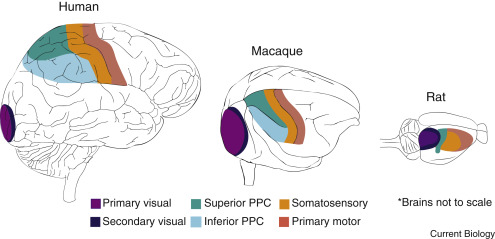
\includegraphics[width=12cm]{graph/brain.jpg}
\caption{Regions of the brain  \cite{Whitlock2017PosteriorPC}}
\end{center}
\end{figure}
\subsection{Blue Brain Project (BBP)}
The Blue Brain Project was founded in May 2005 with the initial goal of creating a simulation of the rat neocortical column. In October of 2015, after various experimentations involving the brain \cite{2013}, the BBP created a first draft of a reconstruction of the neocortical microcircuitry in the somatosensory cortex in a juvenile rat \cite{2015}. This reconstruction contained approximately $31,000$ neurons, where, through patch-clamp studies, there were 55 layer-specific morphological and 207 morpho-electrical neuron sub-types. Through the digital reconstruction, where neurons are positioned according to a restriction to biological bouton densities and number of synapses per connection, their overlapping arbors form approximately 8 million connections from around 37 million synapses \cite{2015}. 

From the BBP website on the construction of the neocortical column, we have results whereupon there are 35 instantiations of a biologically correct model that have been produced. That is, we have 5 rats, with 7 instantiations each, from which there are a further 7 instantiations that take the average of each of the instantiations of the 5 measured rats. We use the data representing the final instantiation, that is labelled as Bio-M in their paper \cite{Reimann_2017}.
\begin{figure}[H]
\begin{center}
\captionsetup{justification=centering}
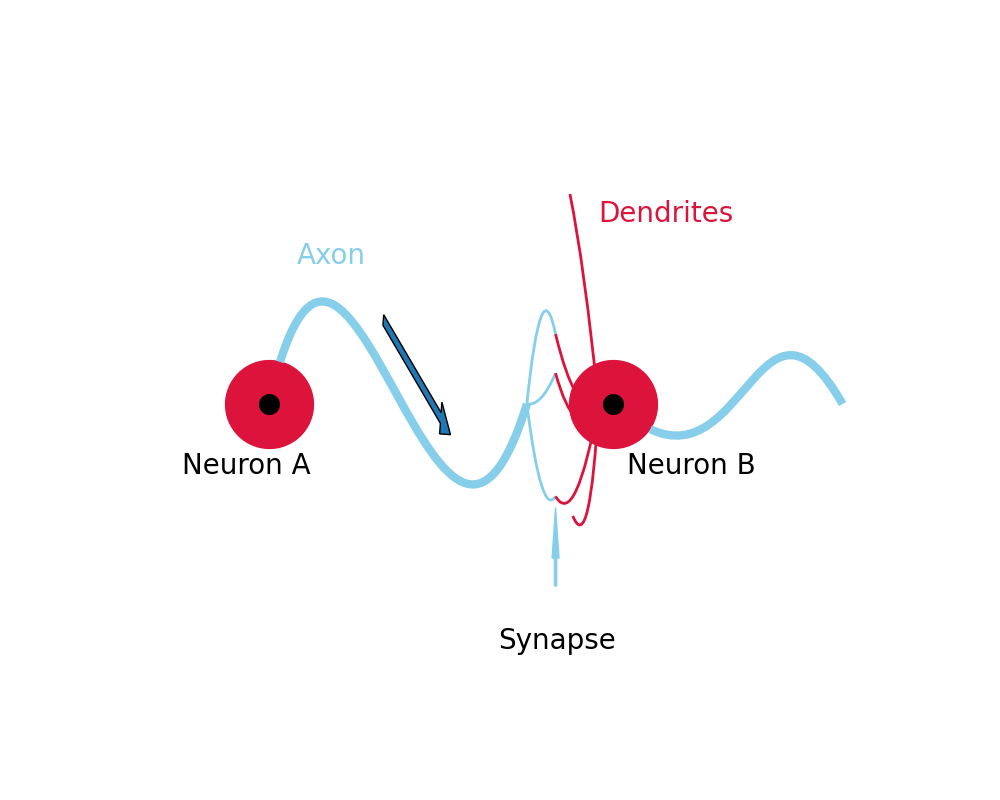
\includegraphics[width=12cm]{graph/cell.png}
\caption{Visual representation of a synaptic connection between two neurons}
\end{center}
\end{figure}
\subsection{Models}
We have four random graph models of the MC plus the \ER model that we wish to compare using topological statistics as to their accuracy in replicating the statistics from the biologically correct model produced by the BBP, the Bio-M MC. The first of these random graph models, is the Configuration model, $\mathcal{G}_{C}$, which rewires the connections between the neurons, without allowing for any self loops while also preserving the in and out degree of each neuron.
Our second random graph model, the Geometric Configuration model, $\mathcal{G}_{GC}$ is identical to the Configuration model while also taking into account the observed distances between connected neurons. 

The third random graph model, the Block Configuration model, $\mathcal{G}_{BC}$, extends the idea of the Configuration model by firstly subdividing the connectome into blocks on a layer by layer basis. We have 6 layers, whereby layers 2 and 3 are considered together. This accounts for 25 blocks. Within each block we have a subset of connected pairwise neurons of the connectome. Each block applies the same connection method as the Configuration model thereafter before being reassembled into a realisation of the connected random graph $\mathcal{G}_{BC}$.


In the final random graph model, the Block Geometric Configuration model, $\mathcal{G}_{BGC}$ we extend the ideas of the previous models,  $\mathcal{G}_{BC}$ and $\mathcal{G}_{GC}$, and combine them. That is to say, we again subdivide the connectome into blocks on the same basis as stated previously for the Block Configuration model, however, this time when we compute a permutation of the connected pairwise neurons in each subset, we take the added constraint of a distance-dependence. Upon completion of a rewiring of each block, we can reassemble the blocks, much like the Block Configuration model, to obtain a realisation of the random graph model $\mathcal{G}_{BGC}$. 





\newpage
\section{Mathematical Preliminaries}
\subsection{Directed Graph}
A directed graph $\mathcal{G}$, consists of a pair of finite sets, $(\emph{V},\emph{E})$. The elements of $\emph{V}$ are the vertices and the elements of $\emph{E}$ are the edges. An edge is a set formed by pairs of vertices. Further to this, there is a function, $\tau$, that associates an ordered pair of vertices for each edge in $\emph{E}$. The direction of an edge $\emph{e} = \{v_1, v_2\}$, is said to be $\tau(\emph{e}) = (v_1, v_2)$, where $\tau_{1}(e) = v_1$ is the source vertex and $\tau_{2}(e) = v_2$ is the target vertex.

With our definitions, there comes a constraint for the function $\tau$.
\begin{itemize}
\item There are no self-loops, that is for each $\emph{e} \in \emph{E}$, if $\tau(\emph{e}) = (v_1, v_2)$ then $v_1 \neq v_2$.
\end{itemize}

There may exist neurons that are reciprocally connected, that is, there may be edges whereby we have $\emph{e}, \emph{e}^\prime \in \emph{E}$ such that $\tau(\emph{e})=(v_1,v_2)$ and $\tau(\emph{e}^\prime) = (v_2,v_1)$.

A vertex $\emph{v} \in \mathcal{G}$ is said to be a sink if there exists no $\emph{e} \in \emph{E}$ such that $\emph{v}=\tau_1(\emph{e})$, but there is at least one edge $\emph{e}^\prime \in \emph{E}$ such that $\tau_2(\emph{e}^\prime) = \emph{v}$. Similarly, \emph{v} is said to be a source if there exists no $\emph{e} \in \emph{E}$ such that $\emph{v} = \tau_2(\emph{e})$, but there is at least one $\emph{e}^\prime \in \emph{E}$ such that $\tau_1(\emph{e}^\prime) = \emph{v}$.

A path in a directed graph consists of a sequence of edges $(e_1, e_2, ..., e_n)$ such that for all $1 \leq k \leq n$, the target of $e_k$ is $e_{k+1}$, i.e.~$\tau_2(\emph{e}_k) = \tau_1(\emph{e}_{k+1})$. The length of the path $(e_1, e_2, ..., e_n)$ is $n$.

If the target of $e_n$ is the source of $e_1$, that is $\tau_2(\emph{e}_n) = \tau_1(\emph{e}_1)$, then $(e_1, ..., e_n)$ is an oriented cycle. A directed graph that contains no oriented cycle is said to be acyclic.

A directed graph is said to be fully connected if for every pair of distinct vertices, there exists a path from one to the other, in at least one direction.
\subsection{Simplices}
A simplex is a generalisation of the notion of a point, a line, a triangle up to some arbitrary dimension. The simplex is named as such since it is the simplest possible polytope in any given space.

We have, for example, the following possible simplices:

\begin{itemize}
    \item A 0-simplex which consists of a vertex.
    \item A 1-simplex which consists of two vertices and an edge with direction.
    \item A 2-simplex which consists of three vertices and three edges all having direction. There is also a clear source and a clear sink. An example is given below.
    \item A 3-simplex consists of 4 vertices and 6 edges all having direction and where we have a clear source and a clear sink.
\end{itemize}
To generalise this, a $k$-simplex is the convex hull of the $k+1$ vertices it contains \cite{2018}.
\begin{figure}[H]%
    \centering
    \captionsetup{justification=centering}
    \subfloat[\centering 0 Simplex]{{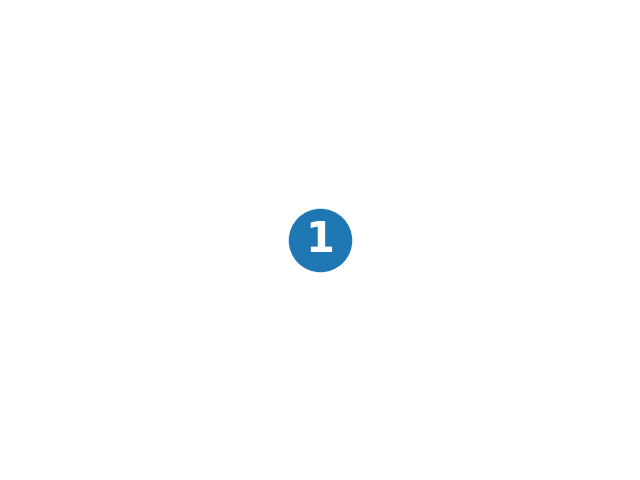
\includegraphics[width=3cm]{graph/0simplex.png} }}%
    \qquad
    \subfloat[\centering 1 Simplex]{{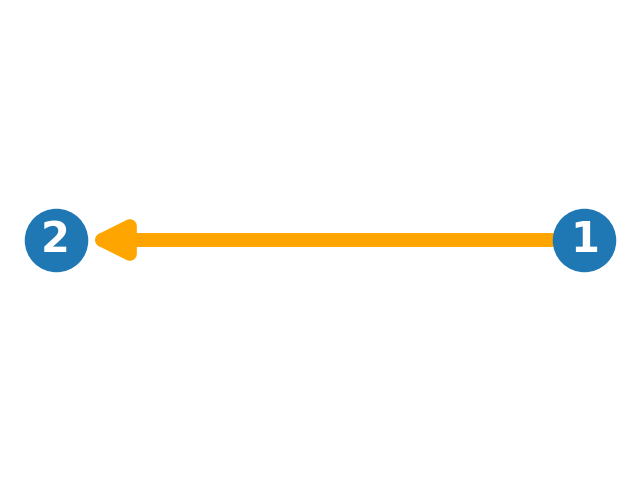
\includegraphics[width=3cm]{graph/1simplex.png} }}%
    \qquad
    \subfloat[\centering 2 Simplex]{{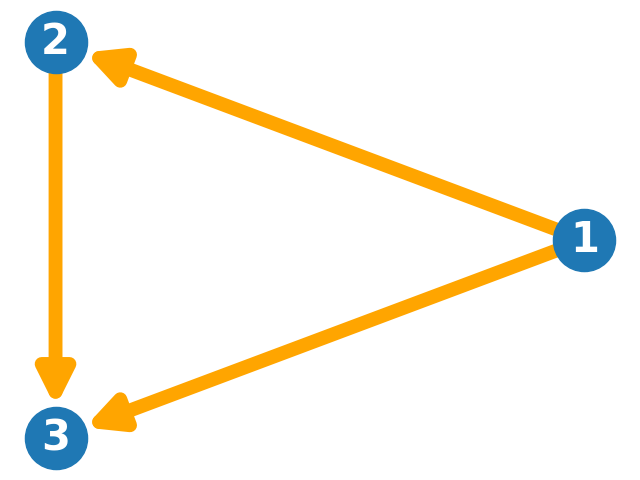
\includegraphics[width=3cm]{graph/2simplex.png} }}%
    \qquad
    \subfloat[\centering 3 Simplex]{{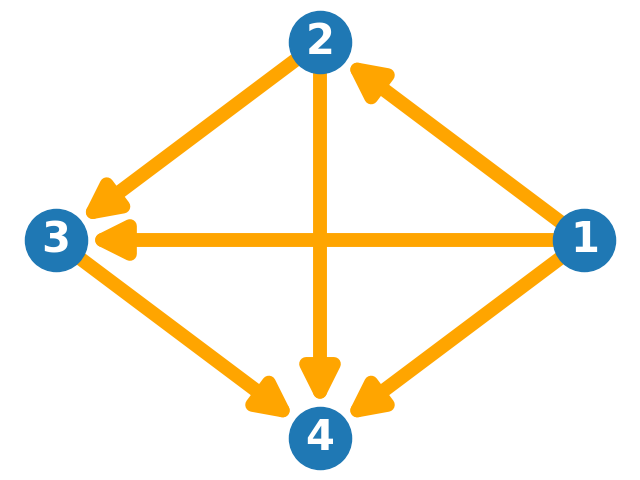
\includegraphics[width=3cm]{graph/3simplex.png} }}%
    \caption{Simplices from dimension 0 through to 3}%
    \label{fig:example}%
\end{figure}

\subsection{Simplicial Complex}
An abstract simplicial complex $\emph{S}$, is a collection of finite sets. These sets are closed under taking subsets, that is, every subset of a set in the family is also in the family. As an example, in a 2 dimensional simplicial complex, we have triangles, which are sets of size 3, their edges, which are sets of size 2 and their vertices which are sets of size 1 \cite{2008Gregarxiv:0809.4221}.

However, we have a slight variation on this in that we have an abstract $\emph{directed}$ simplicial complex. This is where we again have a collection of sets denoted $\emph{S}$. However, this time, the sets are finite and ordered with the property that if $\sigma \in \emph{S}$, then every subset $\tau$ of $\sigma$, with the natural ordering inherited from $\sigma$, is also a member of $\emph{S}$.

The elements $\sigma$ of a simplicial complex $\emph{S}$, are simplices. We define the dimensionality of $\sigma$ to be the cardinality of the set minus one. Therefore, if $\sigma$ is a simplex of dimension $n$, then we refer to $\sigma$ as an $n$-simplex of $\emph{S}$. The set of all simplices of $\emph{S}$ is denoted $\emph{S}_n$. A simplex $\tau$ is said to be a face of $\sigma$ if $\tau$ is a subset of $\sigma$ with a strictly smaller cardinality than $\sigma$. As an example, let's take Figure 3(c). This shows a simplex $\sigma$ of dimension 2, however, we can also consider the edge from vertex 1 to vertex 3 as a face of the 2 dimensional simplex, since this is defined using $\tau$(e) = ($v_1, v_3$) where $\tau$ is a subset of $\sigma$.

These simplices may be joined along these faces. A simplex that is not the face of any other simplex is said to be maximal. Again, with the 2-simplex above, we can see that the maximal dimension of this is 2, and that the edges and vertices that construct this object are faces of the 2-simplex and faces of faces of the 2-simplex respectively. Thus, the set of all maximal simplices of a simplicial complex determines the entire simplicial complex since this is made up entirely of maximal simplicial complexes or a face of a simplicial complex.

\subsection{Simplicial Complex applied to Directed Graphs}
The directed graph $\mathcal{G}$ naturally creates the directed simplicial complex. The directed simplicial complex that is associated to the directed graph $\mathcal{G}$ is called the directed flag complex of $\mathcal{G}$.

The directed flag complex is defined to be the ordered simplicial complex whose $n$-simplices are all ordered $(n+1)$-cliques. So, let it be that $\sigma = (v_0, v_1, ...v_n)$, such that $v_i \in \emph{V}$ for all $i$ and ($v_i, v_j) \in \emph{E}$ for $i < j$. Then the ordered set of these completes the directed flag complex. Further to this, we note that $v_0$ is the initial vertex, or the source of $\sigma$, and that $v_n$ is the final or sink of $\sigma$.

One final thing of note is that because of our assumption on $\tau$, an $n$-simplex in $\emph{S}$ is characterised by the ordered sequence $(v_o, v_1, ..., v_n)$ and not by the vertices. By example, $(v_0, v_1, v_2)$ and $(v_0, v_2, v_1)$ are two distinct 2-simplices that contain the same set of vertices.

\subsection{Directionality}
The directionality \cite{Reimann_2017} of a directed graph $\mathcal{G}$ is given by:
\begin{equation}
    \Dr(\mathcal{G}) = \sum_{v \in V} \sd(\emph{v})^2 \enspace{,}
\end{equation}
where
\begin{equation}
    \sd(\emph{v}) = \Indeg(\emph{v}) - \outd(\emph{v})\enspace{.}
\end{equation}
The signed degree ($\sd$) is given as the in-degree minus the out-degree for each vertex in $\mathcal{G}$. That is, the number of times a given vertex is a target vertex minus the number of times the same given vertex is a source vertex. Following on from this, the directionality of $\mathcal{G}$ is the sum of the squares of all the signed degrees for each vertex in the directed graph $\mathcal{G}$.

Further to this, we can note that the sum of the signed degree for a finite graph is zero. That is,
\begin{equation}
    \sum_{v \in \mathcal{G}}\sd(\emph{v}) = 0 \enspace{.}
\end{equation}

\subsection{Homology}
Simplicial homology arose as a way to study topological spaces. The building blocks of which are our $n$-simplices. On top of this, we have further numerical quantities in order to describe the abstract directed flag complex. These include Betti numbers and the Euler Characteristic. These are described below.

\subsection{Betti Numbers}
Informally, the $k^{th}$ Betti number refers to the number of $k$-dimensional holes on a topological space, where a $k$-dimensional hole is a $k$-dimensional cycle that is not a boundary of a $(k+1)$-dimensional object.

The definitions of the first few Betti numbers are as follows;
\begin{itemize}
    \item $\beta_0$ is the number of connected components
    \item $\beta_1$ is the number of 1-dimensional or `circular' holes.
    \item $\beta_2$ is the number of 2-dimensional `voids' or `cavities'.
\end{itemize}
For example, let's take our triangular prism in Figure 4. We can see that the vertices are all connected as one object. This, as well as with the Bio-M MC, takes the zeroth Betti number to be 1. That is, $\beta_0 = 1$. Next, we take the informal definition of the 1-dimensional Betti number. We can see here that there are no holes that are of dimension 1, so $\beta_1 = 0$. Finally, we look at the second dimensional definition of a Betti number. We are looking for holes or cavities that are entirely enclosed by 2-dimensional objects. We can see that we have a hole that is enclosed by triangles. Therefore, $\beta_2 = 1$. Applying the Euler Characteristic to the Betti numbers of this example, we have,
\begin{equation}
    \beta_0 - \beta_1 + \beta_2 = 1 - 0 + 1 = 2
\end{equation}
So if we take the classical usage of the Euler characteristic, we can see the relationship, as stated above in the Euler characteristic section, is also 2 as follows:
\begin{equation}
    V - E + F = 6 - 8 + 12 = 2
\end{equation}

\begin{figure}[H]%
    \centering
    \captionsetup{justification=centering}
{{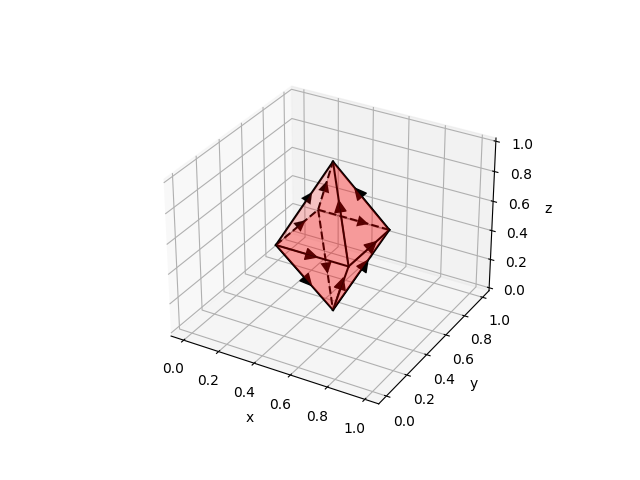
\includegraphics[width=12cm]{graph/simplex_structure.png} }}%
    \caption{Triangular Prism}
    \label{fig:example}%
\end{figure}

Now, informally, let $\mathbb{F}_2$ denote a field of two elements. Let $\emph{S}$ be a simplicial complex. Define the chain complex C*(S, $\mathbb{F}_2$) to be the sequence ($C_n$ = $C_n$(S,$\mathbb{F}_2$))$_{n\geq0}$, such that $C_n$ is the $\mathbb{F}_2$-vector space whose basis elements are the $n$-simplices $\sigma \in  S_n$, for each $n\geq0$. In other words, the elements of $C_n$ are formal sums of $n$-simplices in S.

For each $n\geq1$, there is a linear transformation called a \textit{differential}
\begin{equation}
    \partial_n : C_n \rightarrow C_{n-1} \enspace{.}
\end{equation}
specified by $\partial_n(\sigma) = \sigma^0 + \sigma^1 + ... + \sigma^n$ for every $n$-simplex $\sigma$, where $\sigma^i$ is the $i^{th}$ face of $\sigma$. Having defined $\partial_n$ on the basis, one then extends it linearly to the entire vector space $C_n$. The $n^{th}$ Betti number $\beta_n$(S) of a simplicial complex $\emph{S}$ is the $\mathbb{F}_2$-vector space dimension of its $n^{th}$ mod-2 homology group, which is defined by,
\begin{equation}
    \mathbb{H}_n(\emph{S}, \mathbb{F}_2) = \frac{\Ker(\partial_n)}{ \ime(\partial_{n+1})} \enspace{,}
\end{equation}
for  $n\geq 1$ and
\begin{equation}
    \mathbb{H}_0(\emph{S}, \mathbb{F}_2) = C_0/\ime(\partial_{1}) \enspace{.}
\end{equation}
For all $n\geq1$, there is an inclusion of vector subspaces i.e.~$\ime(\partial_{n+1}) \subseteq \Ker(\partial_{n}) \subseteq C_n$, and thus the definition of homology makes sense.

Computing Betti numbers of a simplicial complex is conceptually very easy. Let $|S_n|$ denote the number of $n$-simplices in the simplicial complex $\emph{S}$. If one encodes the differential $\partial_{n}$ as a $(|\emph{S}_n-1| \times |\emph{S}_n|)$-matrix $D_n$ with entries in $\mathbb{F}_2$, then one can easily compute its \textit{nullity}, null($\partial_n$), and its rank, rk($\partial_n$), which are the $\mathbb{F}_2$ dimensions of the null-space and the column space of $D_n$ respectively. The Betti numbers of $\emph{S}$ are then a sequence of natural numbers defined by,
\begin{equation}
    \beta_0(\emph{S}) = \text{dim}_{\mathbb{F}_2}(C_0) - \text{rk}(\partial_1) \enspace{,}
\end{equation}
\begin{equation}
    \beta_{n}(\emph{S}) = \text{null}(\partial_{n}) - \text{rk}(\partial_{n+1}) \enspace{.}
\end{equation}

Since Im($\partial_{n+1}$) $\subseteq$ Ker($\partial_n$) for all $n\geq 1$, the Betti numbers are always non negative. The $n^{th}$ Betti number $\beta_n$ gives an indication of the n-dimensional cavities in the geometric realisation of S \cite{Reimann_2017}.

\subsection{Euler Characteristic}
The Euler Characteristic is simply defined as the alternating sum of the number of simplices in each dimension. This can also be applied to Betti numbers in each dimension, however, for the Betti numbers for our models and even the \ER model in dimensions 1 through 3, this is not computationally viable since the required memory to compute the Betti numbers in these dimensions is upwards of 16GB.

So, algebraically, the Euler Characteristic is given as follows:
\begin{equation*}
    \chi = k_0 - k_1 + k_2 - k_3 + ...
\end{equation*}
\begin{equation}
    \Rightarrow \chi = \sum_{k \geq 0} (-1)^k \abs{S_k} \enspace{.}
\end{equation}
As a side note, there is a close relationship between the Euler Characteristic and Betti numbers \cite{Reimann_2017}. This relationship is as follows:
\begin{equation}
    \chi(\emph{S}) = \sum_{k\geq 0}(-1)^k \beta_{k}(\emph{S})
\end{equation}


\subsection{Blocks}
Within the MC we have a set of neurons and a set of synapses, represented by vertices and directed edges respectively. Now, when we take into account the direction of information flow, an edge has with it a pair of ordered vertices.

Now, when we subdivide the MC on a layer by layer basis, we are left with 25 subsets of ordered pairs of vertices, each belonging to a ``block''. An example of a block is L1-L4. That is, we have a set of ordered vertices where the pre-synaptic neurons set is from Layer 1 and the post-synaptic neurons are from Layer 4.

This is not to say that there are a specific set of neurons that are pre-synaptic or post-synaptic, but rather, the neuron's state is determined by the order in which it appears in the ordered pair $\emph{e}$.


\subsection{Total Variation distance}
Here, we use the Total Variation (TV) distance to quantify statistical differences between distributions obtained from our models.

Let $f$ and $g$ be two discrete distributions over a common support set $\{1,2,\ldots,n\}$.
Thus, $\sum_{i=1}^{n}f_{i} = 1$ and $\sum_{i=1}^{n}g_{i} = 1$.

Typically, we want to compare distribution $f$ obtained from a model with the distribution $g$ obtained from the Bio-M MC. To compare the distance between these two distributions, we take:
\begin{equation}
\delta(f, g) = \sum_{i=1}^{n}(|f_{i} - g_{i}|)\enspace{.}
\end{equation}

This will output a value in the range $[0, 2]$.
Clearly $\delta(f, g)=0$ if $f=g$ and $\delta(f, g)=2$ if $f$ and $g$ have no common events.

\newpage
\section{The Microconnectome}
Here we introduce the Bio-M MC. This is one of the microcircuits that the BBP reconstructed. It represents the mean measurements of a set of 5 other varying instantiations of a rat's neocortical column.
\subsection{Bio-M MC}
\subsubsection{Origins of the Bio-M MC}
The Blue Brain Project have created multiple variants of a rat's neocortical column (a microconnectome). These are  comprised of 6 sets of 7 statistically varying instantiations. The first 5 of these sets were based on specific heights of the layers in the neocortex. These instantiations ultimately gave rise to a set of average instantiations of the neocortical column. The instance that we focus on here is the final instance in this set of averages, the Bio-M MC. This instance of the neocortical column contains 6 layers, that are made up from a total of 55 different morphological neuron types. These can be further differentiated into excitatory and inhibitory neurons. The Bio-M MC representing the circuit itself contains approximately 7.8 million synaptic connections represented as directed edges that connect the 31,346 neurons represented as vertices.

\begin{figure}[H]
\begin{center}
\captionsetup{justification=centering}
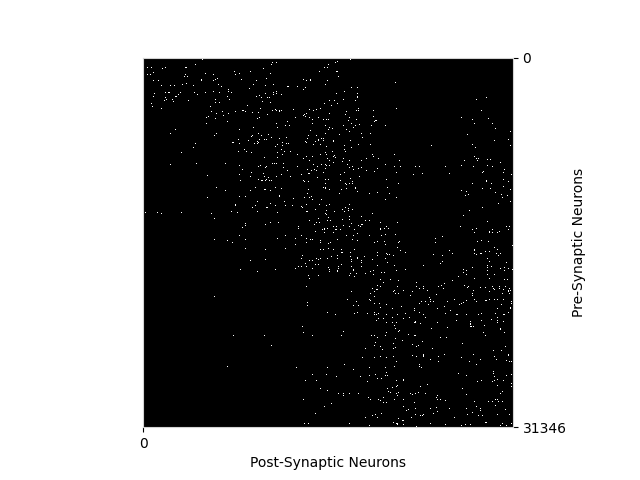
\includegraphics[width=12cm]{BioM/matrix_BioM.png}
\caption{Adjacency Matrix for the Bio-M MC}
\end{center}
\end{figure}
%----------------------
\subsubsection{Block Layout}
\begin{figure}[H]%
    \centering
    \captionsetup{justification=centering}
    \subfloat[\centering Block-wise Edge Densities]{{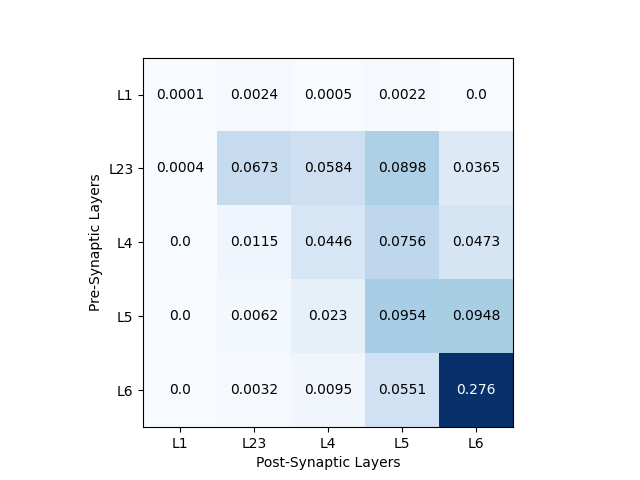
\includegraphics[width=7cm]{BioM/heat_map_layer_BioM_dens_sci.png} }}%
    \qquad
    \subfloat[\centering Block-wise Edge Counts]{{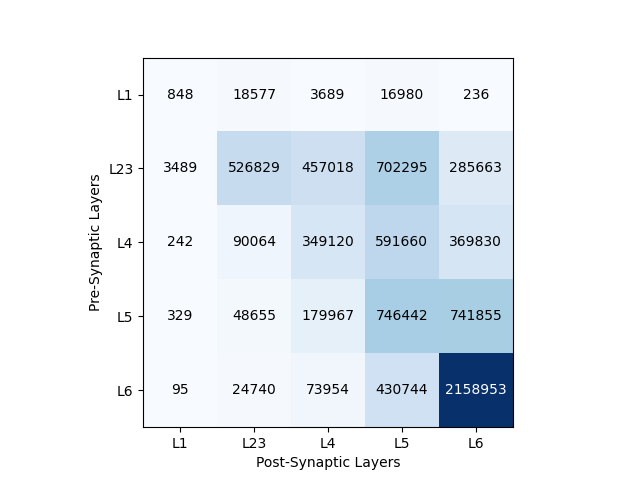
\includegraphics[width=7cm]{BioM/heat_map_layer_BioM.png} }}%
    \caption{Connectivity by block of the Bio-M MC}%
    \label{fig:example}%
\end{figure}

To help visualise the MC, in Figure 5, we have a graphical representation of the connectivity of the neurons as they pass from the pre-synaptic neuron to the post-synaptic neuron in the form of an adjacency matrix. The rows represent the pre-synaptic neurons and the columns represent the post-synaptic neurons. As can be seen here, there is a large number of these connections in the leading diagonal which represents the connections within the layers as compared to off-diagonal blocks that represent connections between the layers, as can be seen in Figure 6. Furthermore, we see that there is a large number of connections that are contained within layer 6. The number of connections in this block amounts to approximately 27\% of all connections in the Bio-M MC.

The volume of the Bio-M MC is approximately $0.29$mm$^3$. The relative thickness is shown in Figure 7, along with statistical details of each layer shown in Table 2.


\begin{center}
\begin{table}[H]
    \centering
    \captionsetup{justification=centering}
     \begin{tabular}{||c | c | c | c||}
 \hline
 Layer & Thickness(\(\mu\)m) & Neurons & Density(neurons/mm\(^3\)) \\ [0.5ex]
 \hline\hline
 1 & 149 & 339 & 14706 \\
 \hline
 2/3 & 502 & 7519 & 31466 \\
 \hline
 4 & 190 & 4661 & 51074 \\
 \hline
 5 & 525 & 6106 & 24214 \\
 \hline
 6 & 700 & 12722 & 37838 \\
 \hline
 \hline
\end{tabular}
    \caption{Statistical details of the Bio-M MC}
    \label{tab:my_label}
\end{table}

\end{center}
\begin{figure}[H]
\begin{center}
\captionsetup{justification=centering}
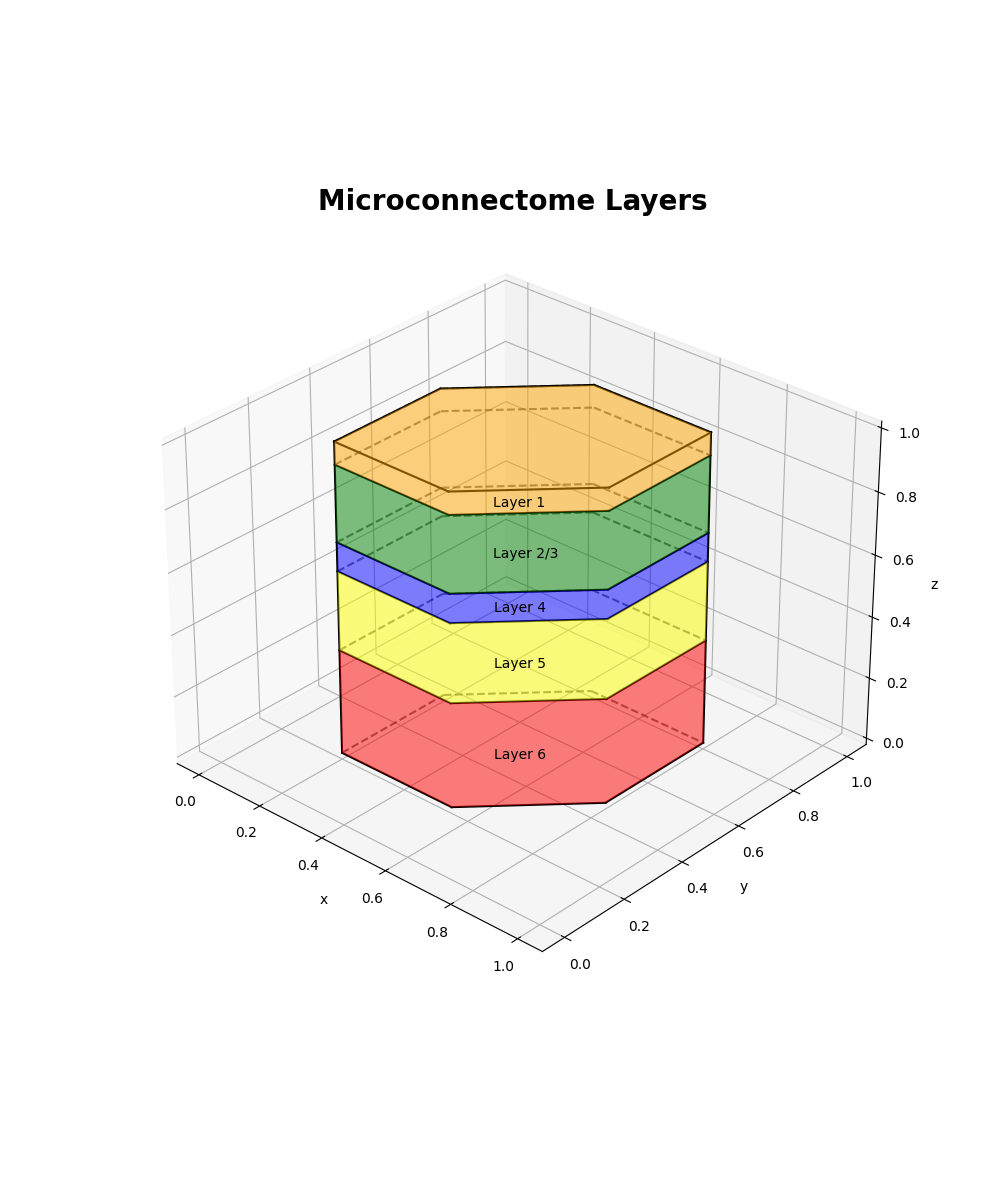
\includegraphics[width=10cm]{BioM/connectome.png}
\caption[center]{Neocortical column scaled to account for layer thickness}
\end{center}
\end{figure}



\subsubsection{Distance Distribution}
To see further how the models compare to the original structure of the Bio-M MC, we also want to take a look at distances between the connected neurons to see how much of an impact distance has on the level of connectivity within the MC. Since our models are only dealing with the neurons and the observed synaptic connections that are present in the Bio-M MC, we look only at the functional graph, as shown in Figure 8.

\begin{figure}[H]
\begin{center}
\captionsetup{justification=centering}
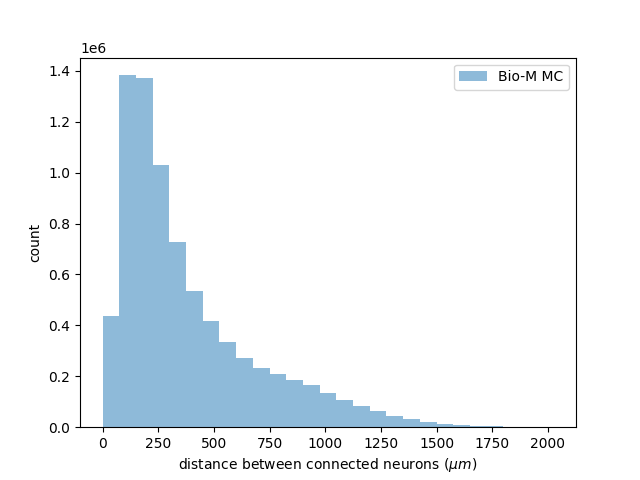
\includegraphics[width=10cm]{BioM/BioM_dist_distr.png}
\caption{Distance distribution of connected neurons in the Bio-M MC}
\end{center}
\end{figure}

We have taken the bin sizes to be 75\(\mu\)m, to be consistent with the distances that were proposed in \cite{Reimann_2017}. This is due to 75$\mu$m being the maximum bin size that preserved the distribution of soma-distances of connected neurons in all sub-matrices of the adjacency matrix representation of the MC. A sub-matrix here, is defined by the connections between a morphological neuron type and another morphological neuron type. For example, we have L1 DAC to L1 HAC. This is just one example of the 3025 sub-matrices that are contained in the MC. More details of this are given in the section on the General Biological model.

\subsubsection{Signed Degree of Neurons}
In Figure 9, we have the signed degree of the neurons. These are calculated by taking the neurons in-degree minus the out-degree. Therefore, a positive value as shown in Figure 9(a), indicates that the information flow into the neuron is greater than the flow out and vice versa for a negative degree. So, from Figure 9(a), we can see that more flow is directed towards the neurons that are located in layers 1, 2 and 3 and that more flow moves away from the neurons in layers 4, 5 and 6. This, theoretically, is down to the fact that L4 is the major thalamorecipient layer and therefore a starting point of cortical information processing. Subsequently, information is then propagated through the cortical column, firstly to L2/3, then from there to L5 and L6, which are the primary output layers of the cortex \cite{10.3389/fnana.2017.00091}.

To show that the graph representing the network is finite, we can take the sum of signed degree for each neuron over the set of neurons, $\sum_{v \in \mathcal{G}}\sd(\emph{v}) = 0 \enspace{.}$ Figure 9(b) shows the cumulative sum of the signed degree of each neuron throughout the MC. All models barring the \ER model follow this pattern as we aim to preserve this.

\begin{figure}[H]%
    \centering
    \captionsetup{justification=centering}
    \subfloat[\centering Signed Degree of each neuron in Bio-M MC]{{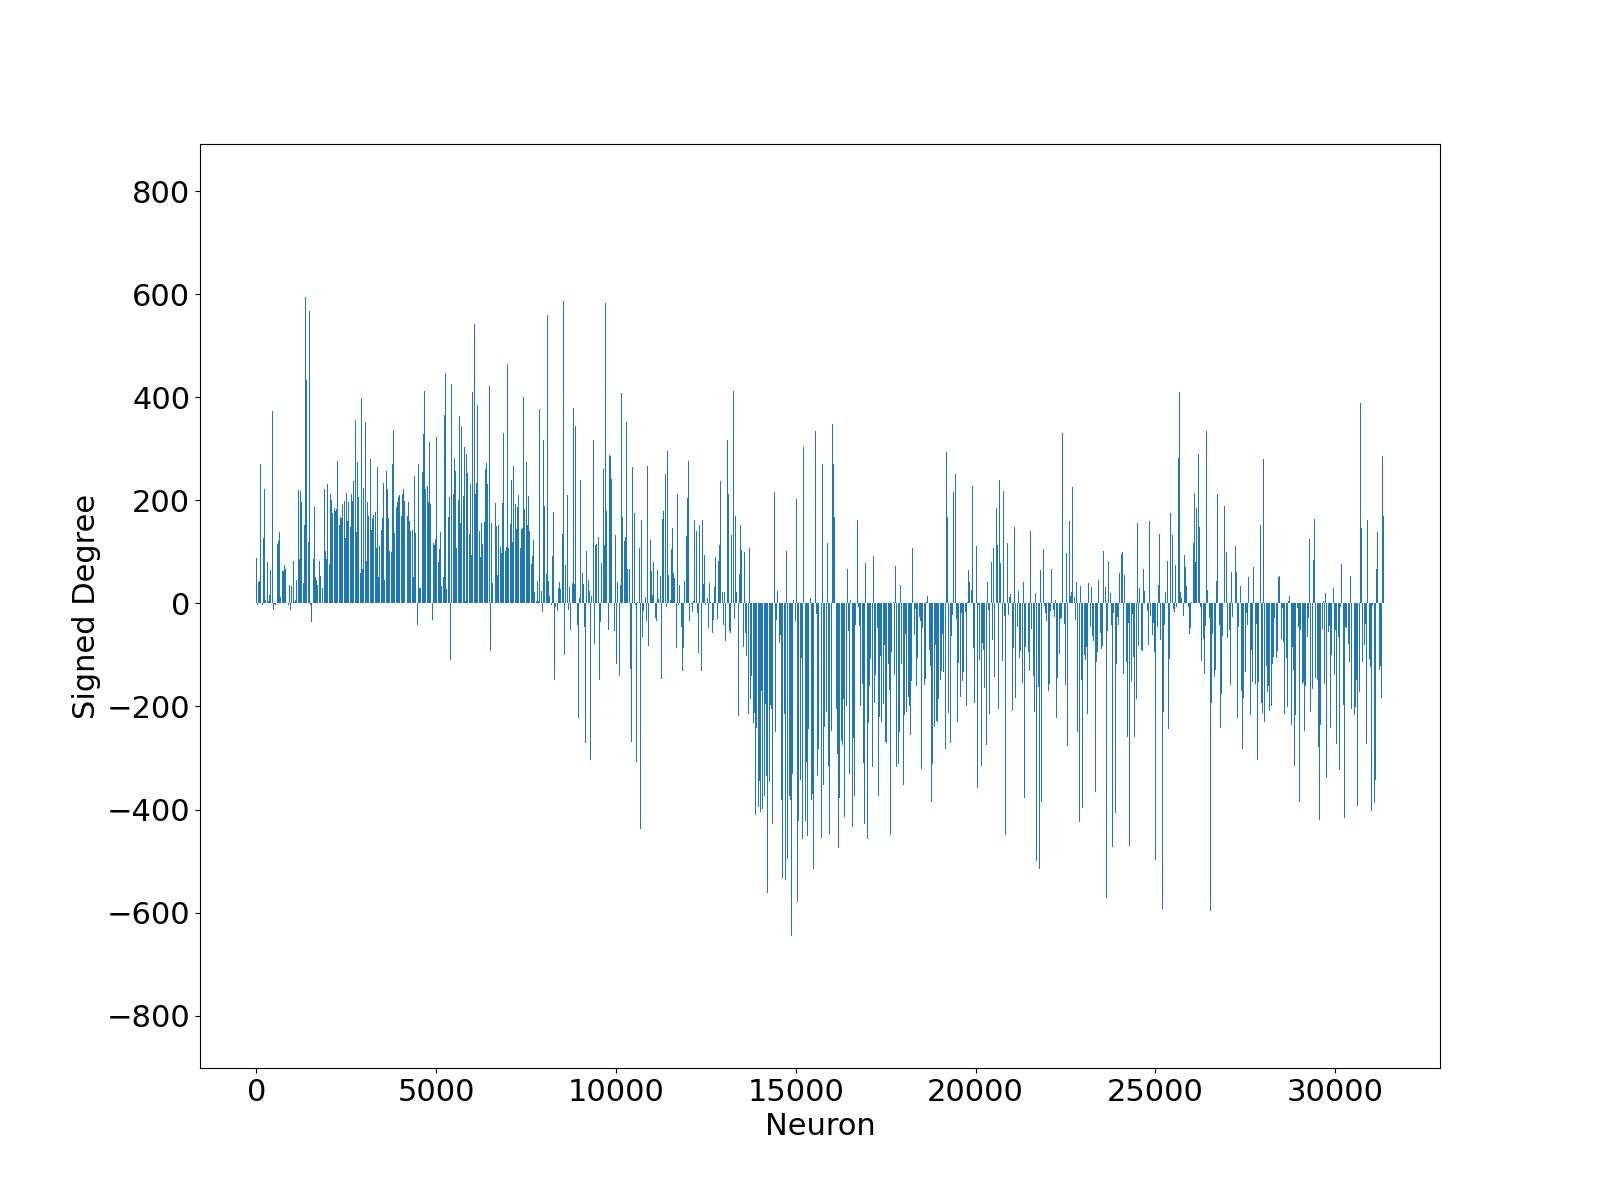
\includegraphics[width=7cm]{BioM/BioM_sd.png} }}%
    \qquad
    \subfloat[\centering Cumulative sum of signed degree to show graph $\mathcal{G}$ is finite]{{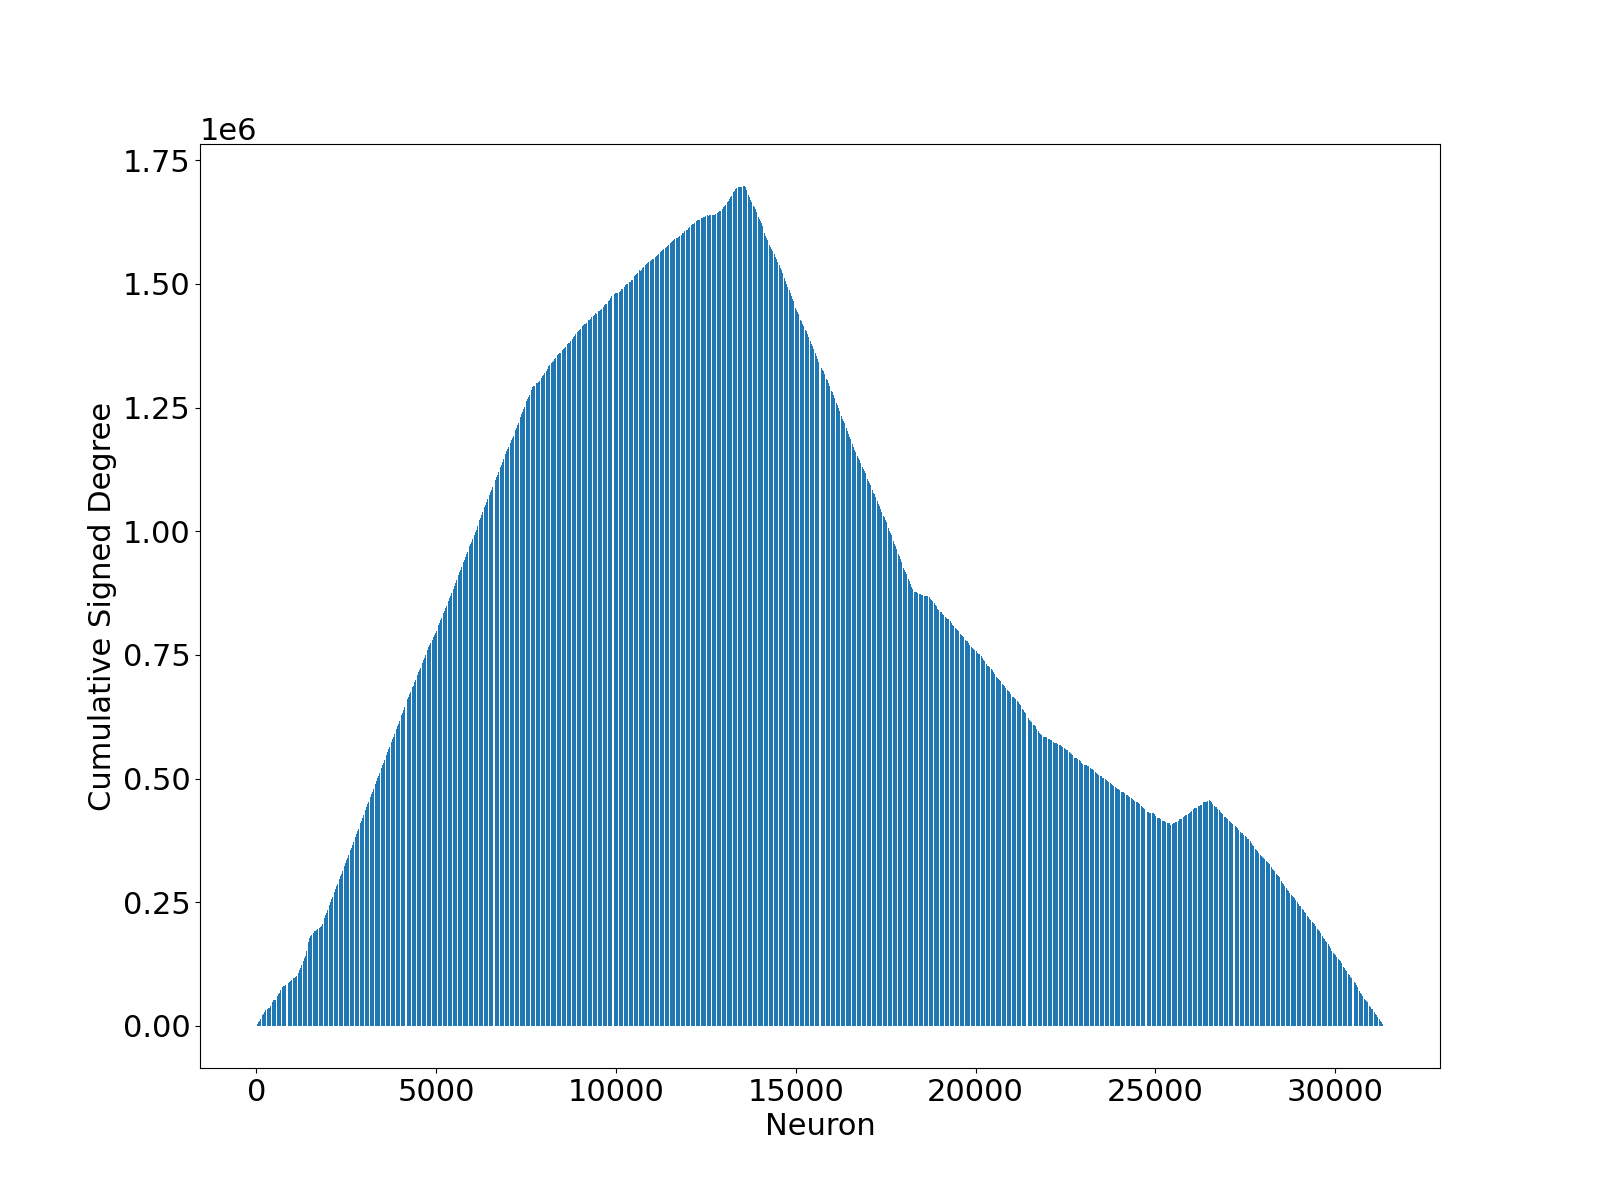
\includegraphics[width=7cm]{BioM/cumsum_degree_BioM.png} }}%
    \caption{Signed Degree statistics for the Bio-M MC}%
    \label{fig:example}%
\end{figure}

\newpage
\section{Models for the Microconnectome}
In this section, we study the Random Graph models with regards to how well they capture the various properties of the Bio-M MC. We fit the parameters of the Random Graph models to the Bio-M MC.
\subsection{\ER Model}
\subsubsection{Construction}
As a starting point for the modelling of the MC, we first construct the \ER random graph model. To be consistent with the statistics of the Bio-M MC, we restricted this model to contain 31,346 neurons and approximately 8 million synaptic connections. To achieve this for the \ER random graph model, we set each potential connection between any pair of neurons to be ~0.8\%, that is;

\begin{equation}
    P(e) =\frac{|\textrm{E}|}{|\textrm{V}|^{2}} = \frac{7,822,274}{31,346^2} \approx 0.8\%
\end{equation}
where e is an edge, $|E|$ is the total number of connections and $|V|$ is the total number of neurons in the Bio-M MC. We typically let the vertex set of labelled neurons to be $V = \{0, 1, 2, \dots, |V|-1\}$

\begin{algorithm}[H]
\SetAlgoLined
\SetKwInOut{Input}{Input}
\SetKwInOut{Output}{Output}
\Input{Vertex Set V, $p \leftarrow 0.008$, random number generator \textit{r} $\in[0, 1)$}
\Output{Adjacency Matrix $M$}
\Init{}{
$M[i,j] \leftarrow 0~~\forall~ (i,j) \in V \times V$}
\ForEach{$i,j \in V \times V$}{\If{r $<$ p}{M[i,j] $\leftarrow$ 1}}
\caption{$\mathcal{G_{ER}} (V, p, r)$}
\end{algorithm}

\begin{figure}[H]
\begin{center}
\captionsetup{justification=centering}
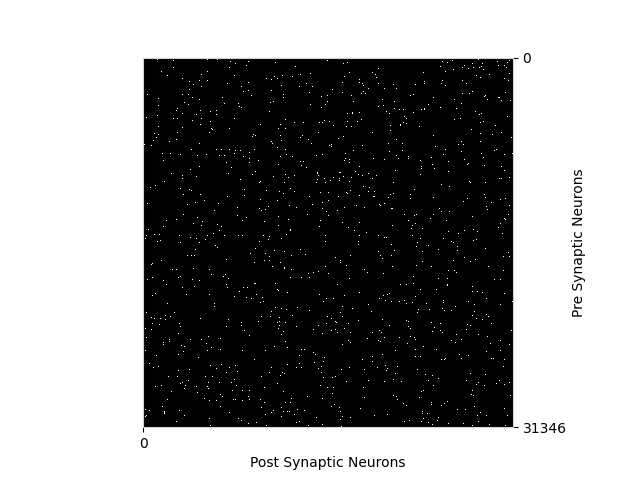
\includegraphics[width=12cm]{ER/matrix_Erdos-Renyi.png}
\caption{Sample output from the \ER model based on the statistics of the Bio-M MC}
\end{center}
\end{figure}
\subsubsection{Block Layout}
Given that each neuron pairing has an equal probability of connecting, it is unsurprising that a sample from $\mathcal{G}_{ER}$, shown in Figure 10, gives a uniform distribution of connections contained within each block. To illustrate this fact further, in Figure 11, we see each block contains approximately $0.8\%$ of the total potential connections within that block. This type of illustration where we speak purely in terms of the number of potential connections in each block is dealt with for this model only. The subsequent models in later sections will deal with Block-Wise Edge Densities with respect to the proportion of connections observed in the functional graph created by the Bio-M MC. We look at this for the \ER model now.
Given the distribution of edges in the blocks of the MC, it becomes clear that the block sizes are unequal. We can see this clearly from and 12(b), where we observe that each block contains a varying number of connections, ranging from around 900 to 1.2 million connections. Figure 12(a) gives the Block-Wise Edge Densities. A breakdown of the TV distance of the Block-Wise Edge Densities from the Bio-M MC can be found in section 6.4.
\begin{figure}[H]
\begin{center}
\captionsetup{justification=centering}
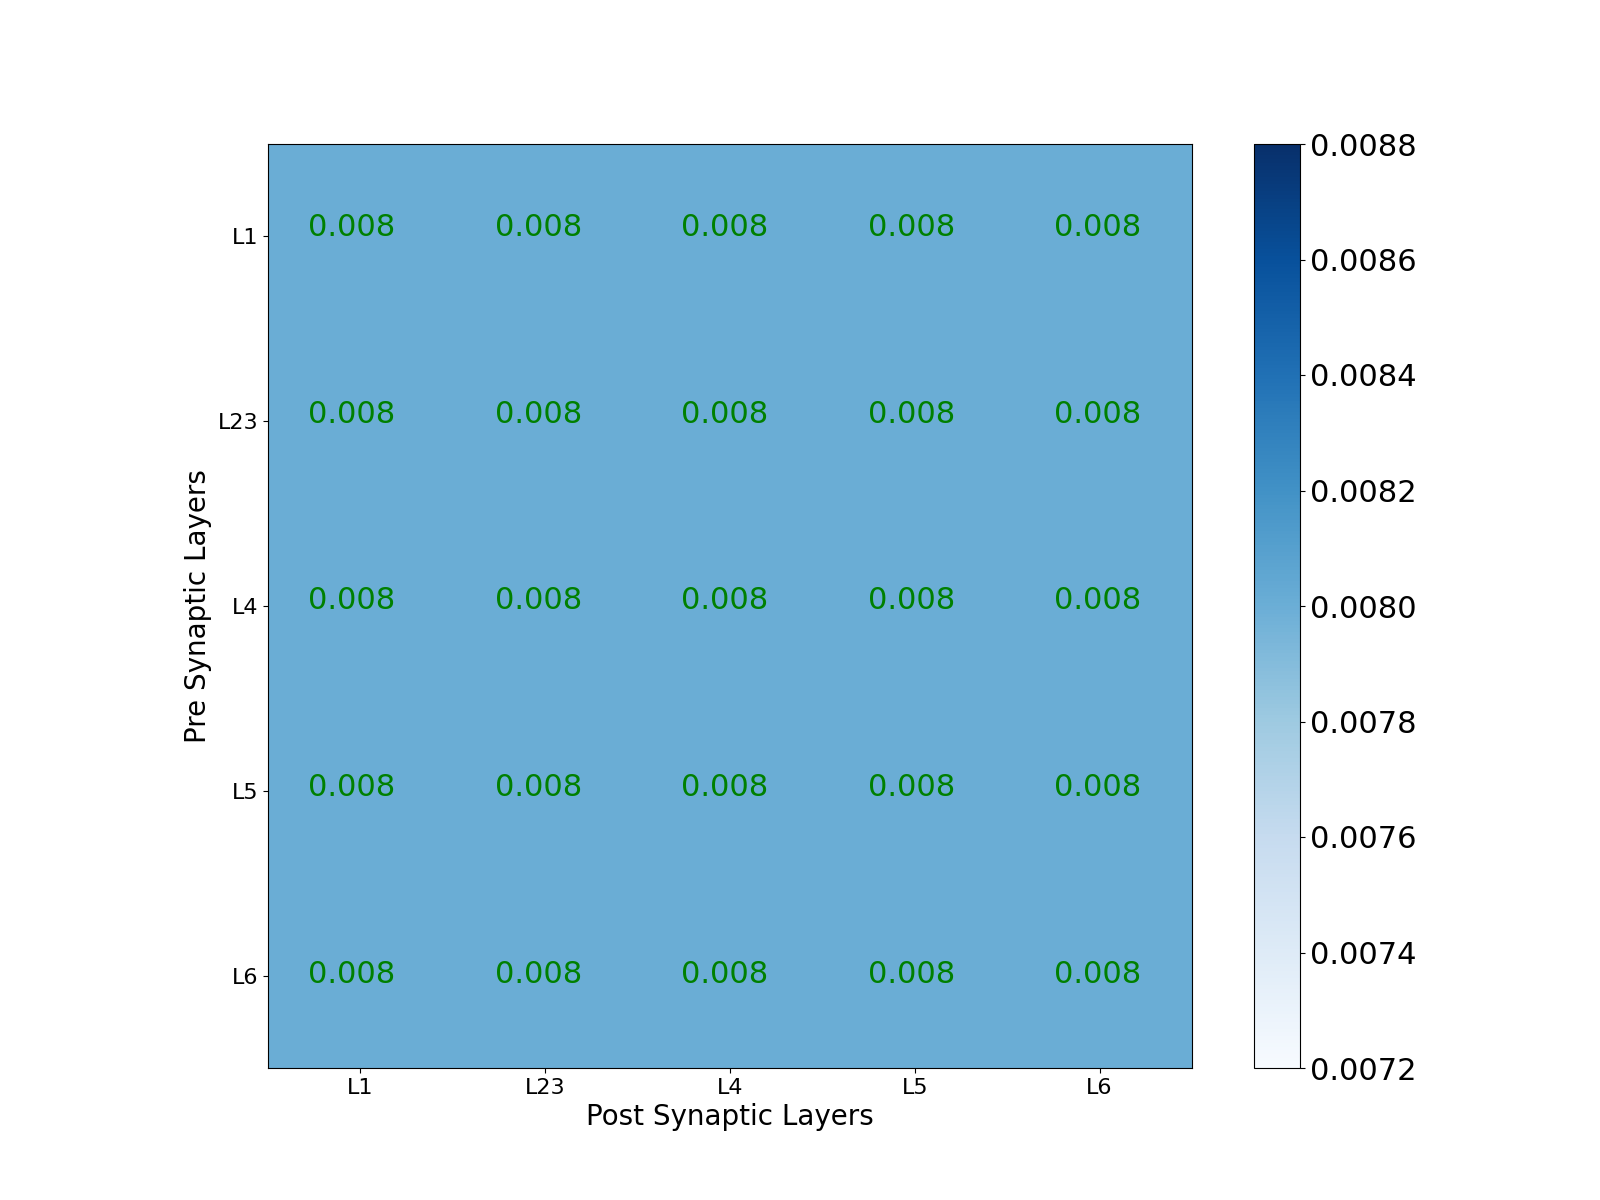
\includegraphics[width=9cm]{ER/heat_map_layer_Erdos-Renyi probability.png}
\caption{Density of edges in each block: $\frac{\text{Edges in block}}{\text{Total number of potential edges}}$}
\end{center}
\end{figure}


\begin{figure}[H]%
    \centering
    \captionsetup{justification=centering}
    \subfloat[\centering Block-Wise Edge Densities ]{{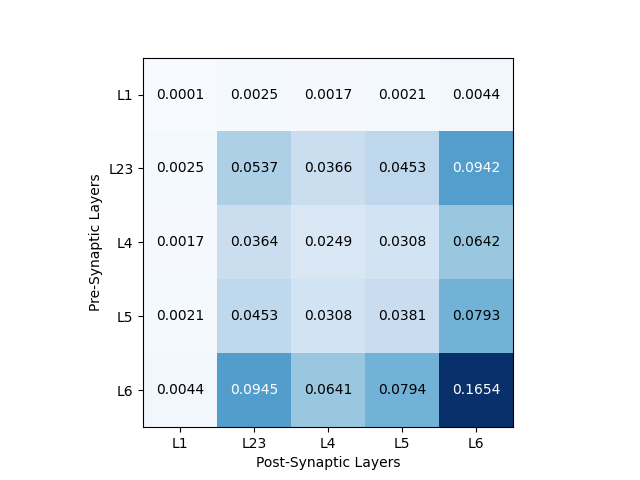
\includegraphics[width=7cm]{ER/heat_map_layer_er_test.png} }}%
    \qquad
    \subfloat[\centering Block-Wise Edge Counts]{{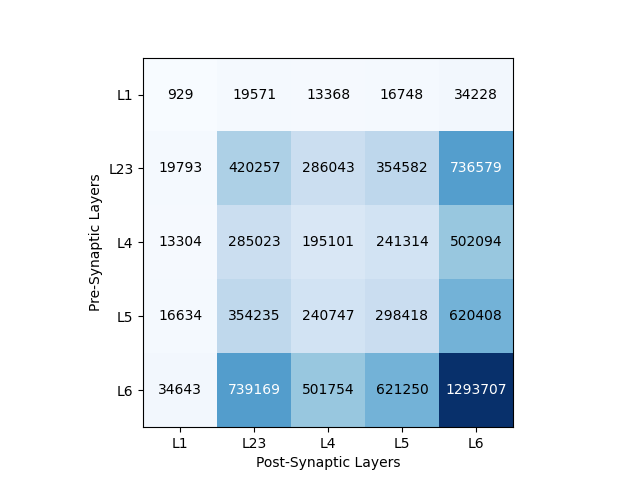
\includegraphics[width=7cm]{ER/heat_map_layer_Erdos_Renyi.png} }}%
    \caption{Connectivity by block of a random graph $\mathcal{G}_{ER}$ given by the \ER model}%
    \label{fig:example}%
\end{figure}

\subsubsection{Distance distributions}
To get an idea of the distribution of distances between neurons under the \ER model, we superimposed it onto that of the functional graph of the Bio-M MC. We computed the pairwise distances of the indexed neurons and plotted the histogram to represent these connections against what it was for the Bio-M MC in Figure 13. A metric that we use to ascertain differences here, is that of the TV distance, described in mathematical preliminaries, between the \ER model and the Bio-M MC. Here, briefly, we can state that, over 100 realisations, the mean TV distance between the \ER model and the Bio-M MC is 0.7092. This is the highest distance between a model and the MC described here. Further details about this statistic are to be found in Section 6, Results.
\begin{figure}[H]
\begin{center}
\captionsetup{justification=centering}
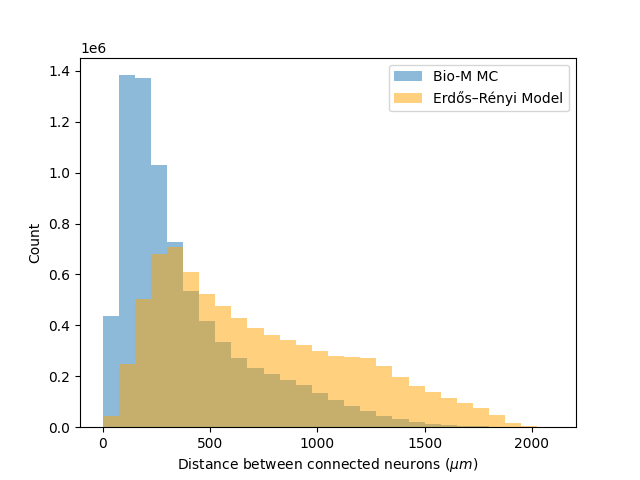
\includegraphics[width=9cm]{ER/Erdos_Renyi_dist_distr.png}
\caption{Distance distribution of connected neurons for the random graph $\mathcal{G}_{ER}$ \\if they were superimposed onto functional graph of the Bio-M MC}
\end{center}
\end{figure}

\subsubsection{Signed Degree of Neurons}
One noteworthy difference between the \ER random graph model and all the other models, as can be seen from the cumulative signed degree graphs in Figure 14, is that each neuron does not maintain the same in-degree and out-degree as that of the Bio-M MC and therefore all of our other models that preserve the in-degree and out-degree of the Bio-M MC.

\begin{figure}[H]%
    \centering
    \captionsetup{justification=centering}
    \subfloat[\centering Realisation 1 ]{{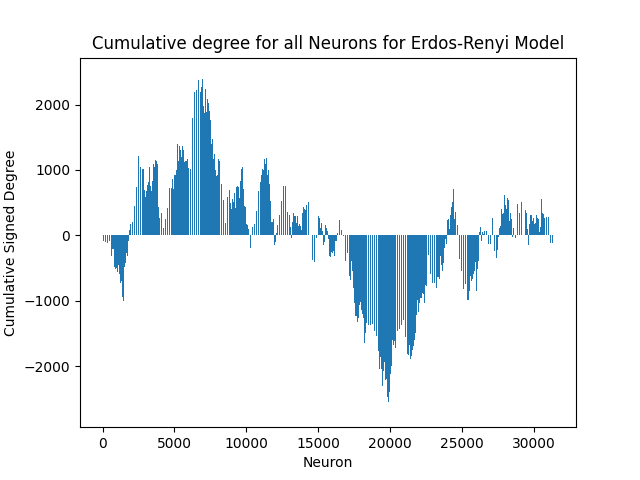
\includegraphics[width=7cm]{ER/cumsum_degree_Erdos-Renyi.png} }}%
    \qquad
    \subfloat[\centering Realisation 2]{{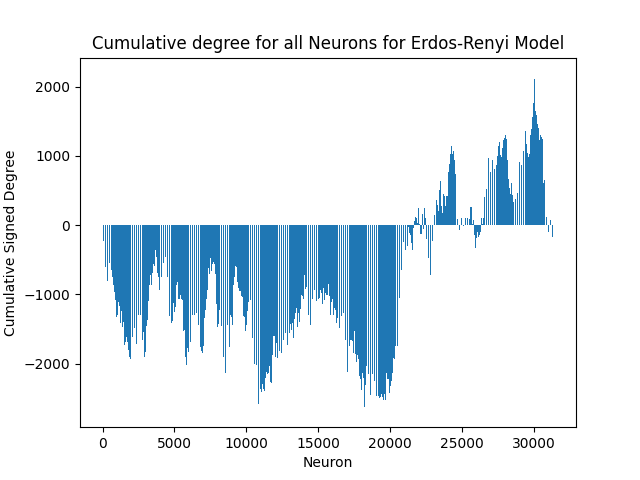
\includegraphics[width=7cm]{ER/cumsum_degree_Erdos-Renyi1.png} }}%
    \qquad
    \subfloat[\centering Realisation 3]{{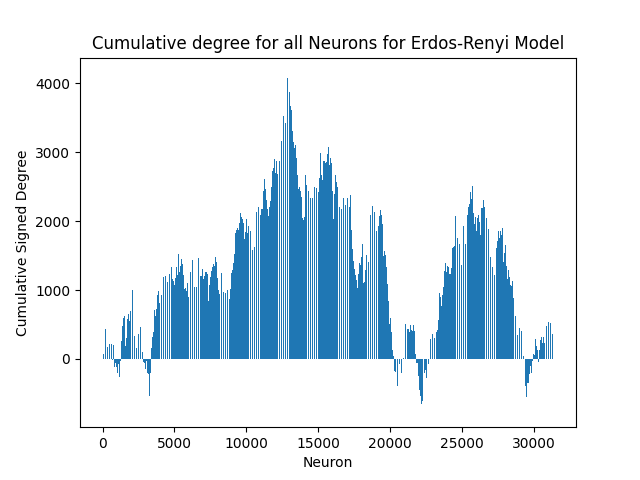
\includegraphics[width=7cm]{ER/cumsum_degree_Erdos-Renyi2.png}}}%
    \qquad
    \subfloat[\centering Realisation 4]{{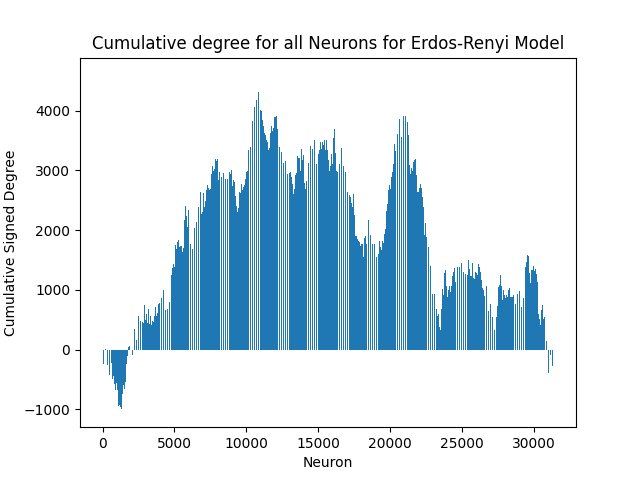
\includegraphics[width=7cm]{ER/cumsum_degree_Erdos-Renyi3.png}}}
    \caption{Realisations of the Cumulative Signed Degree for \ER random graph model}%
    \label{fig:example}%
\end{figure}










\newpage


%--------------------------------------
%--------------------------------------
%--------------------------------------
\subsection{Configuration Model}
This model reconnects the Bio-M MC using the ``cut-permute-rewire'' algorithm proposed by Watts and Strogatz \cite{WattsStrogatz1998}.

\subsubsection{Construction}
We use the ``cut-permute-rewire'' algorithm to produce samples from $\mathcal{G}_{C}$, the Configuration random graph model. This model outputs the rewired neurons by a  resampling of the connected directed edges of the Bio-M MC. By restricting ourselves to the constraints of the algorithm, this model will be able to retain the same in-degree and out-degree for each vertex as the Bio-M MC. One difference to the Bio-M MC and the General Biological model (mentioned later) however, is that we exhibit multiple connections that occur between a pair of neurons that traverse in the same direction. We allow these connections to exist so as to ensure that each neuron does indeed maintain its in-degree and out-degree. This occurs for the subsequent three models as well, namely the Geometric Configuration model, the Block Configuration model and the Block Geometric Configuration model.


\begin{figure}[H]%
    \centering
    \captionsetup{justification=centering}
    \subfloat[\centering Before configuration of small network]{{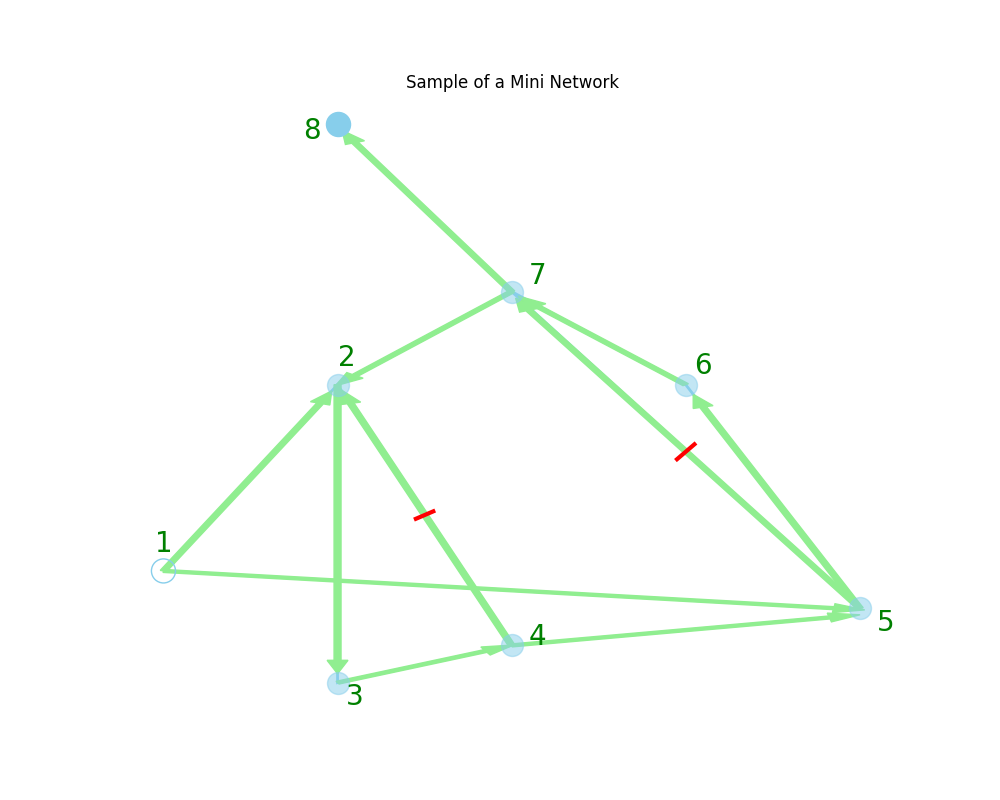
\includegraphics[width=7cm]{configuration/config_before_rewire.png} }}%
    \qquad
    \subfloat[\centering After configuration of network]{{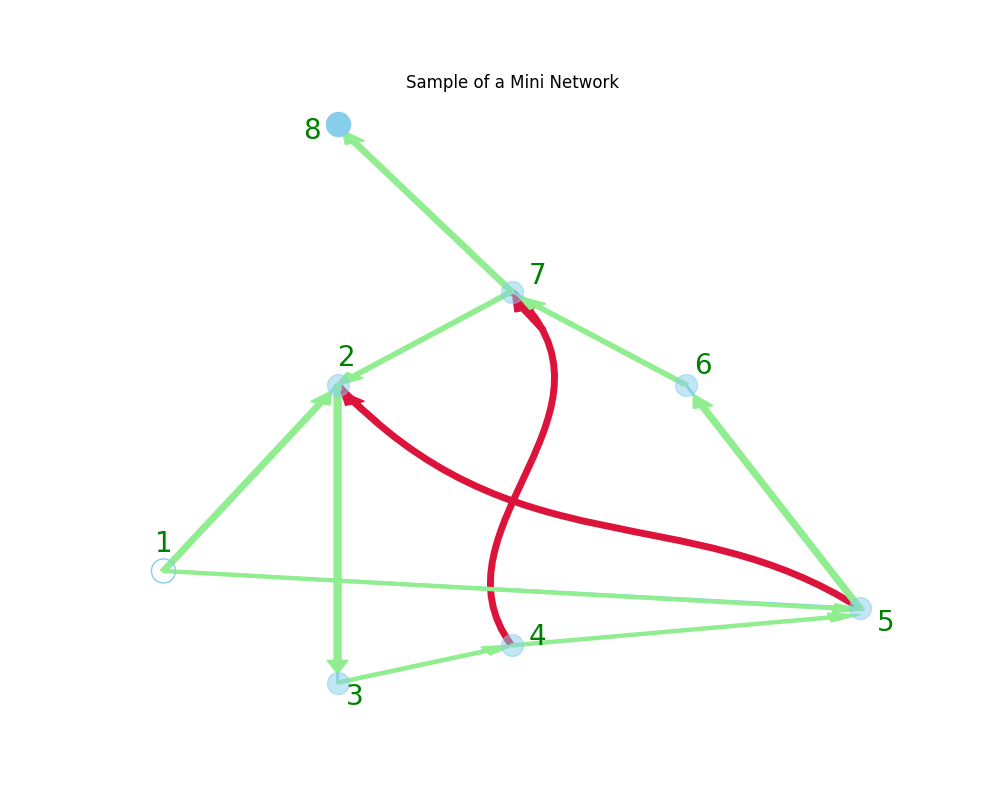
\includegraphics[width=7cm]{configuration/config_after_rewire.png} }}%
    \caption{Example of a configuration of a small version of the network}%
    \label{fig:example}%
\end{figure}

\begin{algorithm}[H]
\DontPrintSemicolon
\SetAlgoLined
\SetKwInOut{Input}{input}
\SetKwInOut{Output}{output}
\SetKwData{$E$}{$(u, v)$}
\Input{$u$, $v$}
\Output{Adjacency Matrix $M$}
\Init{}{$u \leftarrow$ Shuffle($u$)\\
$M[i,j] \leftarrow 0~\forall (i,j) \in [u][v]
$}

\ForEach{$(i,j) \in [u][v]$}
{\eIf{$i \neq j$}{$M[i,j] \leftarrow 1$}{$u \leftarrow$ Shuffle($u$)}}
\caption{$\mathcal{G_{C}}$(u, v)}
\end{algorithm}

For the ``cut-permute-rewire'' \cite{WattsStrogatz1998} algorithm to run, we first take the ordered set of edges in E, where we assign, for each $e \in E$, $\tau_1(e) = v_1$ as the pre-synaptic neurons represented by $u$ in Algorithm 2, and assign $\tau_2(e) = v_2$ as the post-synaptic neurons, represented as $v$ in Algorithm 2. We then initialise the algorithm by shuffling the order of $u$ so as to obtain a permutation of $u$, the pre-synaptic neurons. We then attempt to connect each vertex pairing providing we do not have the same vertex, that is $i \neq j$, to avoid self-loops. If we happen upon an occurrence of this, then we reshuffle the remaining vertices in $u$ and continue. Upon completion, we acquire a new ordered set of vertices contained in $u^\prime$. With this new ordered set of vertices in $u^\prime$, and the vertices in $v$, we can then form the adjacency matrix $M$ that represents a realisation of the random graph model $\mathcal{G}_{C}$.

\begin{figure}[H]
\begin{center}
\captionsetup{justification=centering}
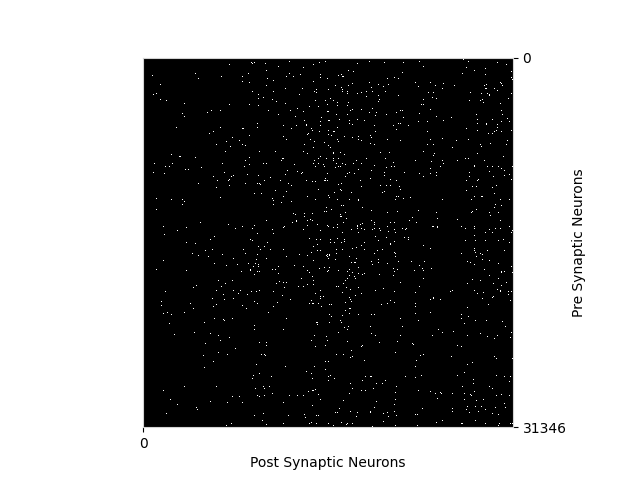
\includegraphics[width=12cm]{configuration/matrix_configuration.png}
\caption{Adjacency matrix $M$ representing a realisation of the random graph $\mathcal{G}_{C}$}
\end{center}
\end{figure}
\subsubsection{Block Layouts}
In Figure 17, we have a breakdown of the Block-Wise Edge connections, both in terms of counts and in terms of density of connections within the functional graph. The density of connections concerning layer 1 amount to less than $1\%$ of all connections in a realisation of the random graph model $\mathcal{G}_{C}$ of the MC. Similarly, in relation to the structure of the Bio-M MC functional graph, the highest number of connections occur in the self-contained block of layer 6 to layer 6. Further statistics on the TV distance of the Block-Wise Edge Densities between the models can be found in Section 6, Results.

\begin{figure}[H]%
    \centering
    \captionsetup{justification=centering}
    \subfloat[\centering Block-Wise Edge Densities]{{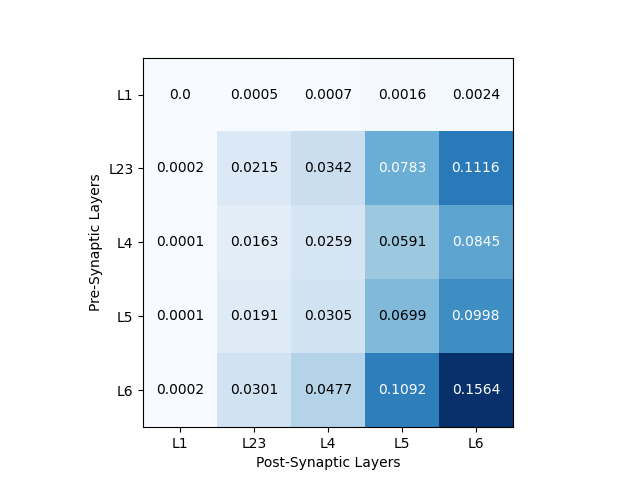
\includegraphics[width=7cm]{configuration/heat_map_layer_c_test.png} }}%
    \qquad
    \subfloat[\centering  Block-Wise Edge Counts]{{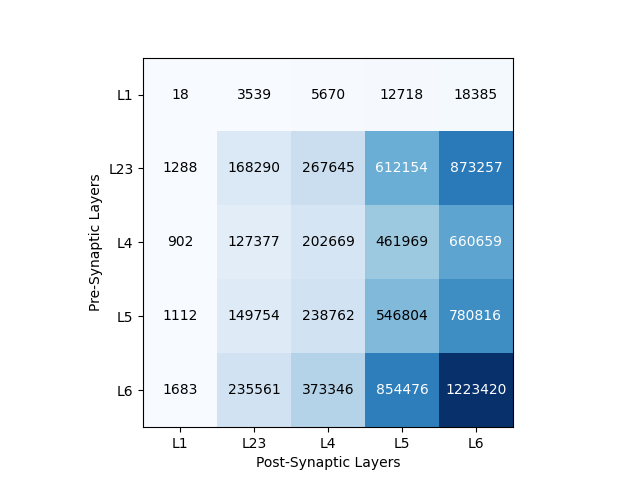
\includegraphics[width=7cm]{configuration/heat_map_layer_configuration.png} }}%
    \caption{Connectivity by block of the random graph $\mathcal{G}_{C}$ given by the Configuration Model}%
    \label{fig:example}%
\end{figure}
\subsubsection{Distance Distributions}
In Figure 18, we can also see a similar distance distribution as to that of the \ER model. As mentioned for the \ER model, we have a TV distance to the Bio-M MC. For the Configuration model, this is 0.6595. This is an improvement on the TV distance given by the \ER model. Further details are given in the Results section.
\begin{figure}[H]
\begin{center}
\captionsetup{justification=centering}
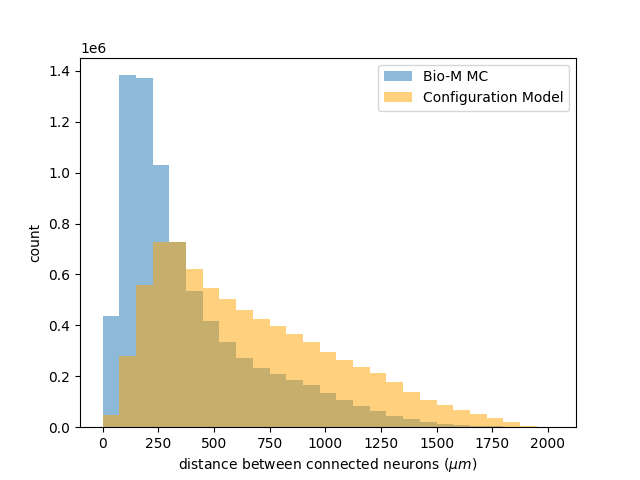
\includegraphics[width=12cm]{configuration/configuration_dist_distr.png}
\caption{Distance distribution of connected neurons for the random graph $\mathcal{G}_C$}
\end{center}
\end{figure}
\subsubsection{Signed Degree of Neurons}
From Figure 19, we see that the each neuron has maintained its in-degree and out-degree thereby following the constraints of the ``cut-permute-rewire'' \cite{WattsStrogatz1998} algorithm.
\begin{figure}[H]%
    \centering
    \captionsetup{justification=centering}
    \subfloat[\centering Signed degree of each neuron ]{{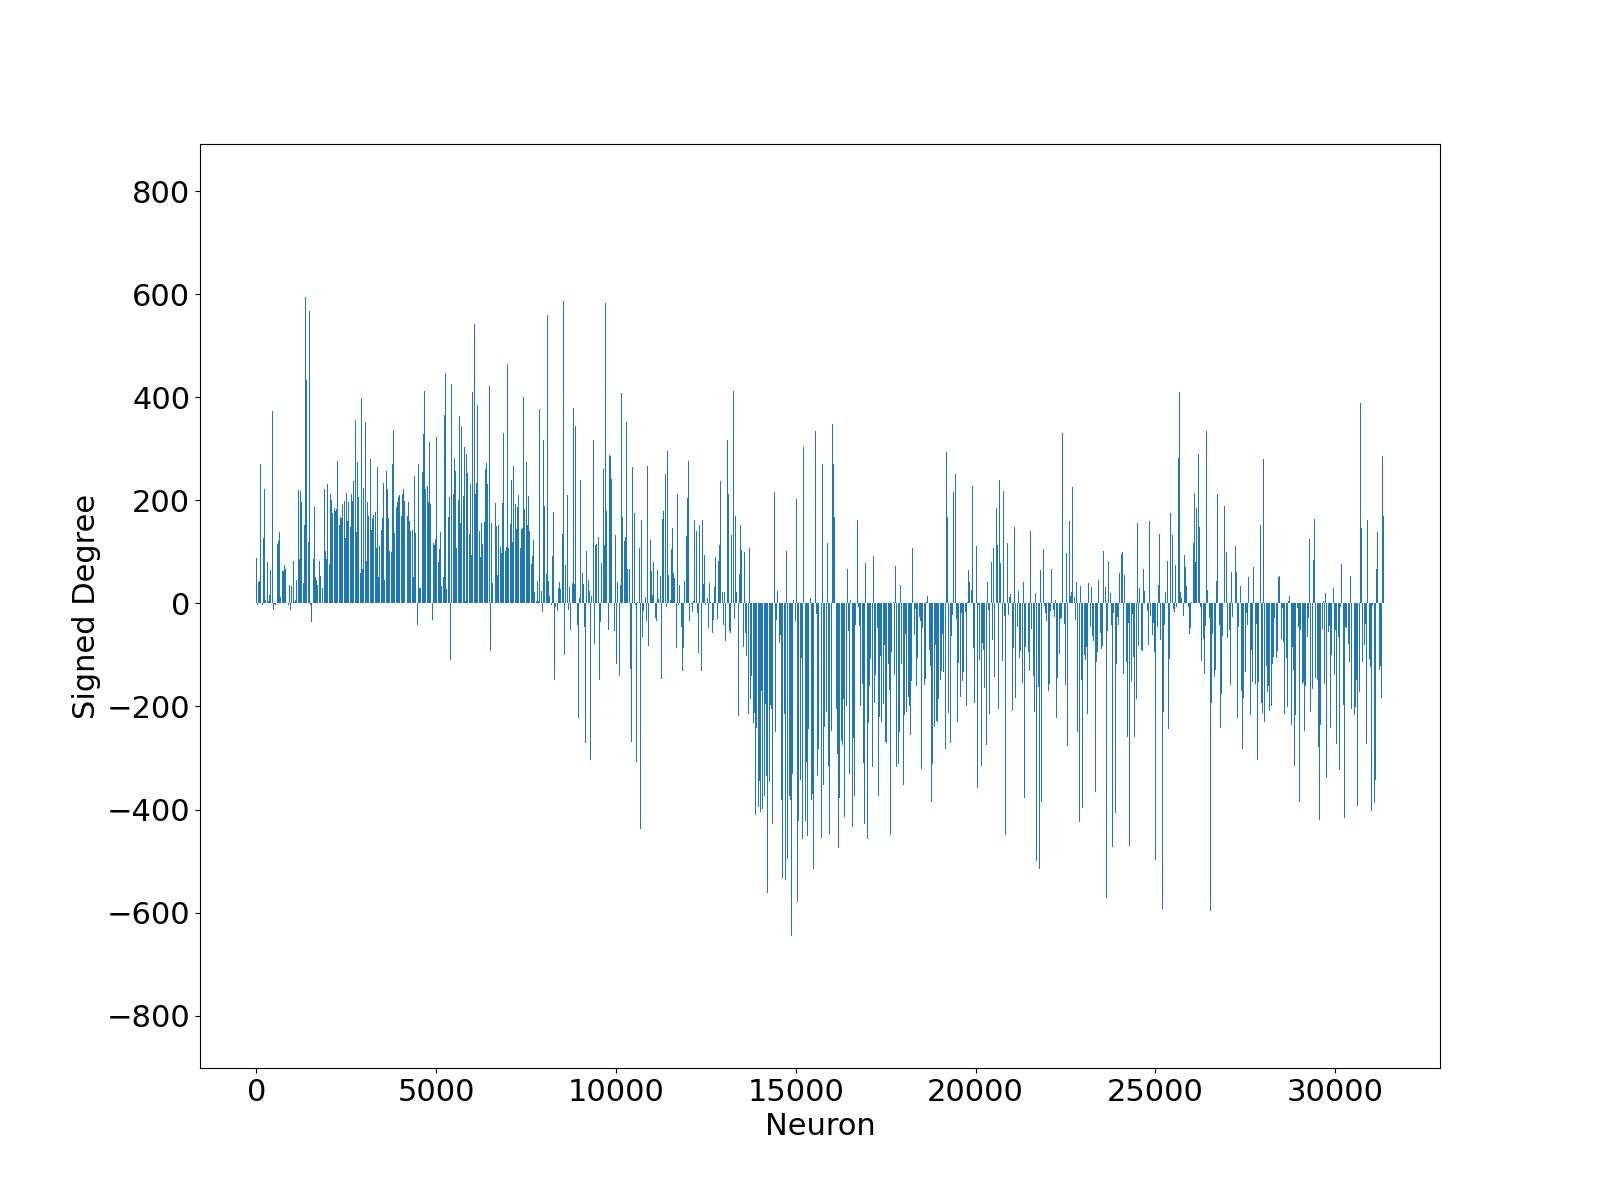
\includegraphics[width=7cm]{configuration/configuration_sd.png} }}%
    \qquad
    \subfloat[\centering Cumulative sum of the Signed Degree of the neurons in a realisation of the random graph $\mathcal{G}_{C}$]{{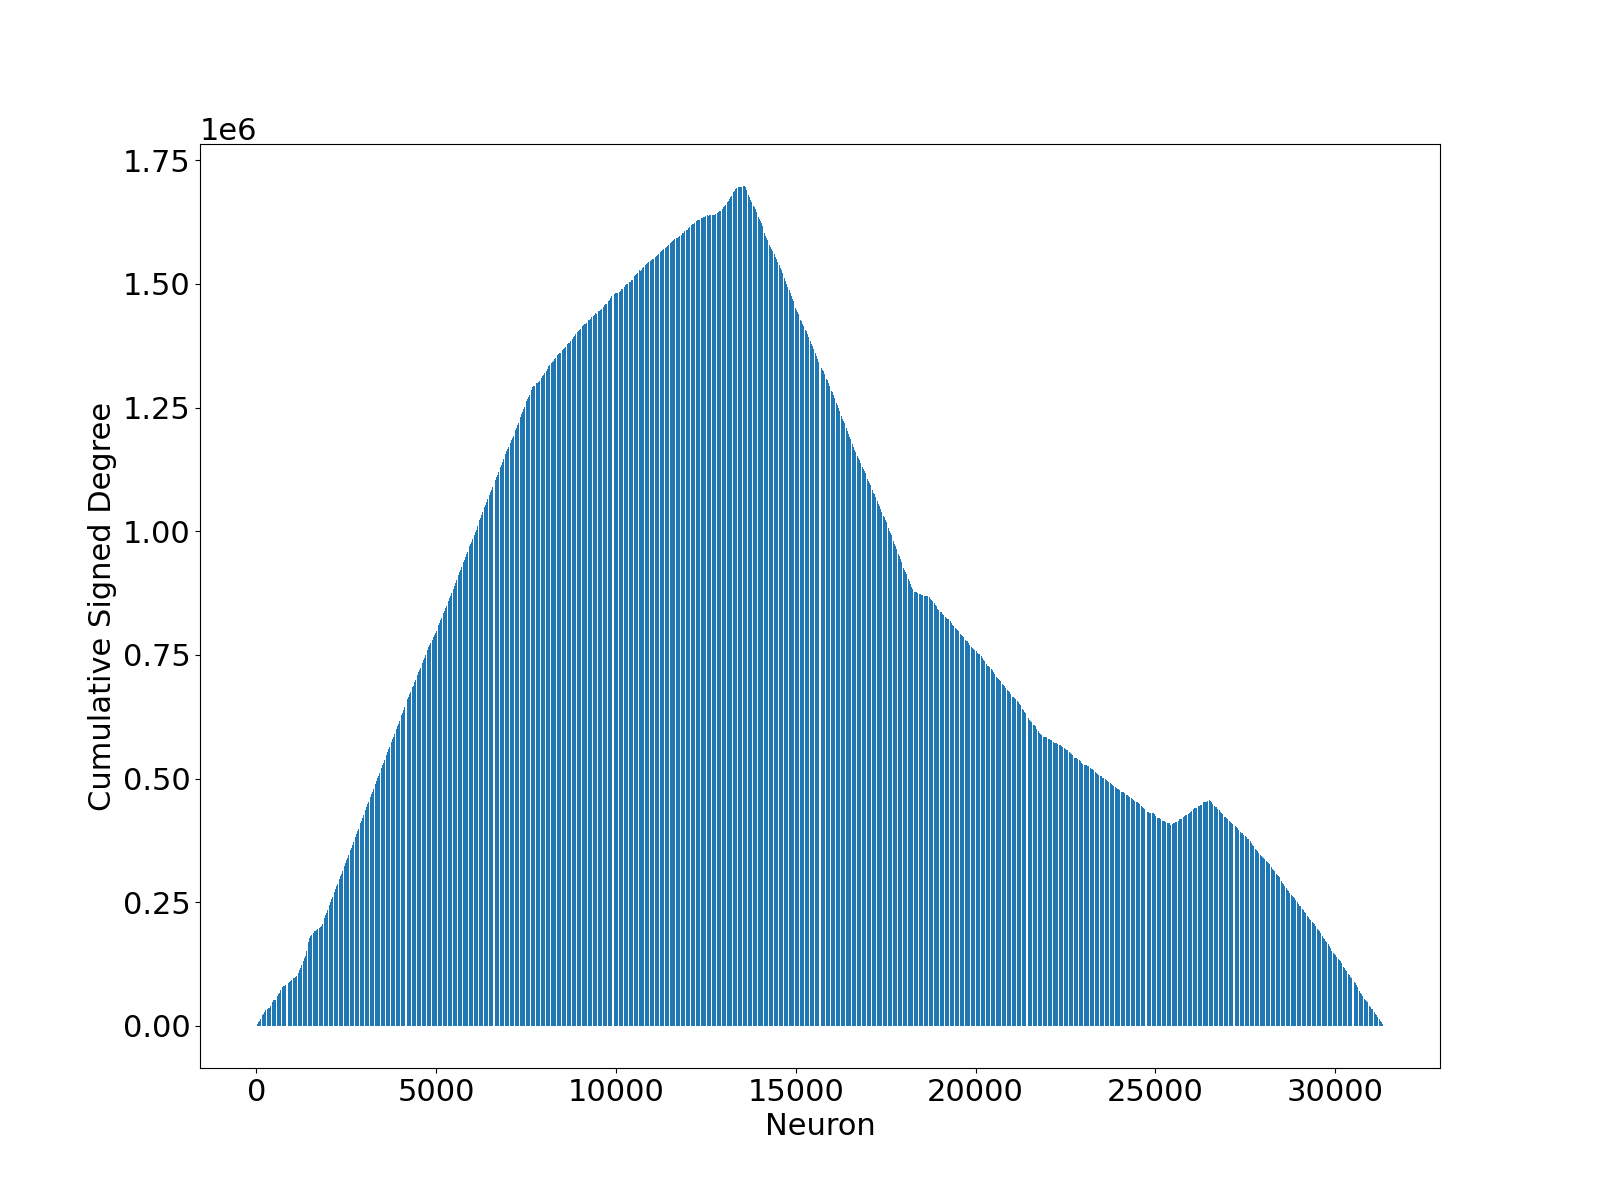
\includegraphics[width=7cm]{configuration/cumsum_degree_configuration.png} }}%
    \caption{Neuron Statistics for a realisation of the random graph $\mathcal{G}_C$}%
    \label{fig:example}%
\end{figure}



%-------------------------------------
%-------------------------------------
%-------------------------------------
\newpage
\subsection{Geometric Configuration Model}
We introduce the Geometric Configuration (GC) model here. This model uses the distances between the connected neurons in the Bio-M MC. The GC model applies the ``cut-permute-rewire'' \cite{WattsStrogatz1998} algorithm to the connected neurons in the Bio-M MC, whilst also considering a geometric constraint of their distances from one another.
\subsubsection{Construction}
The GC model is a variation of the Configuration model. This model has the added constraint that we must also take into account the locations of the neurons, in particular their pairwise distances, involved in the Bio-M MC. In Algorithm 3, we use a probability value p, that is determined by the distance distribution given in Figure 8.

\begin{algorithm}[H]
\SetAlgoLined
\SetKwInOut{Input}{input}
\SetKwInOut{Output}{output}
\SetKwData{$E$}{$(u, v)$}
\Input{$u$, $v$, $p$, random number generator $r$}
\Output{Adjacency Matrix $M$}
\Init{}{$u \leftarrow$ Shuffle($u$)\\
$M[i,j] \leftarrow 0~\forall (i,j) \in [u][v]
$}

\ForEach{$(i, j) \in [u][v]$}
{\eIf{$i \neq j$ \textbf{and} $r < p$}
{$M[i,j] \leftarrow 1$}
{$u \leftarrow$ Shuffle($u$)}}
\caption{$\mathcal{G}_{GC}$(u, v, p) using cut-permute-rewire}
\end{algorithm}

\begin{figure}[H]
\begin{center}
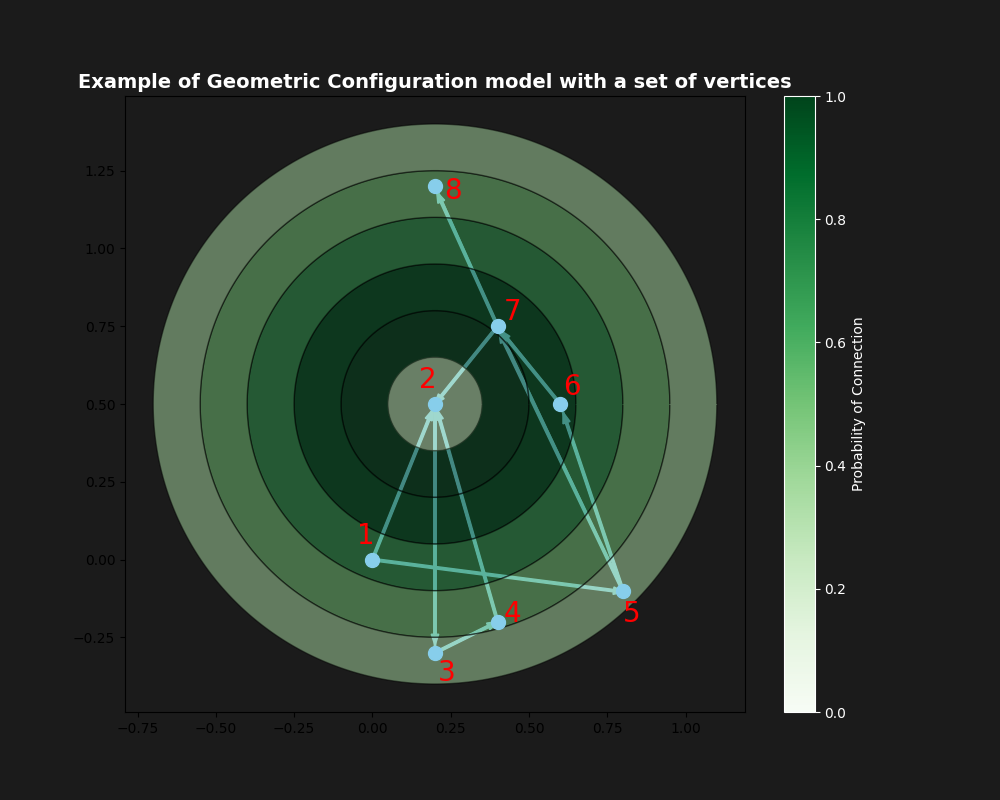
\includegraphics[width=12cm]{GC/gc_example.png}
\caption{Example of a collection of neurons and their varying probabilities of connection with neuron 2}
\end{center}
\end{figure}
As a note on the random graph model $\mathcal{G}_{GC}$, we compute the pairwise distance between each pair of vertices in $E$, whereby we obtain the distance distribution shown in Figure 8. This distribution shows the absolute counts of pairwise distances between neurons. This is then normalised to be used as the empirical probability distribution for connection probability between two neurons based on their pairwise distance.
There are occasions whereby a pair of neurons may contain multiple connections heading in the same direction and that these are included in order to make sure we maintain the same in-degree and out-degree for each neuron.
\begin{figure}[H]
\begin{center}
\captionsetup{justification=centering}
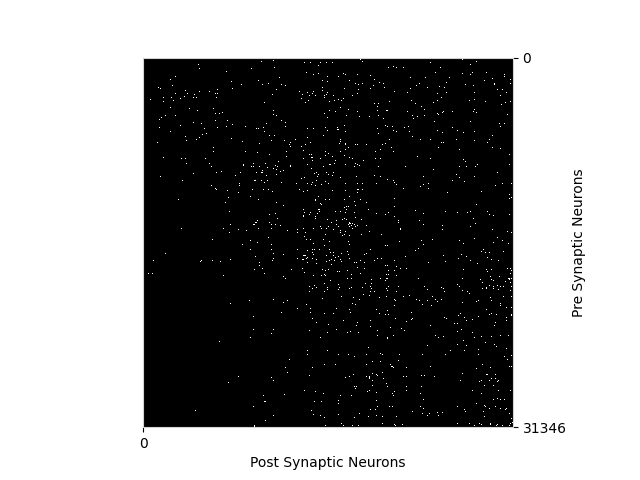
\includegraphics[width=12cm]{GC/matrix_GC.png}
\caption{Adjacency matrix $M$ of a realisation of the random graph $\mathcal{G}_{GC}$}
\end{center}
\end{figure}
\subsubsection{Block Layouts}
Figure 22 gives the breakdown of Block-Wise Edge connections, again, both in terms of counts and in terms of densities of the functional graph. Once again, we can see a small proportion of edges are contained in layer 1 and that the vast majority of edges are within layer 6. The TV distance of the Block-Wise Edge Densities resulted in a similar distribution of values to the Configuration Model relatively speaking. However, the vast majority of blocks here observed smaller TV distances than the Configuration Model, by a factor of 10 or more. Further details can be found in Section 6, Results.

\begin{figure}[H]%
    \centering
    \captionsetup{justification=centering}
    \subfloat[\centering Block-Wise Edge Densities]{{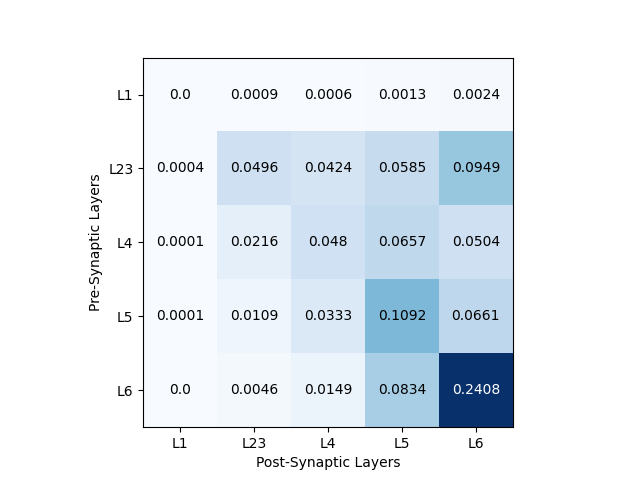
\includegraphics[width=7cm]{GC/heat_map_layer_gc_test.png} }}%
    \qquad
    \subfloat[\centering Block-Wise Edge Counts]{{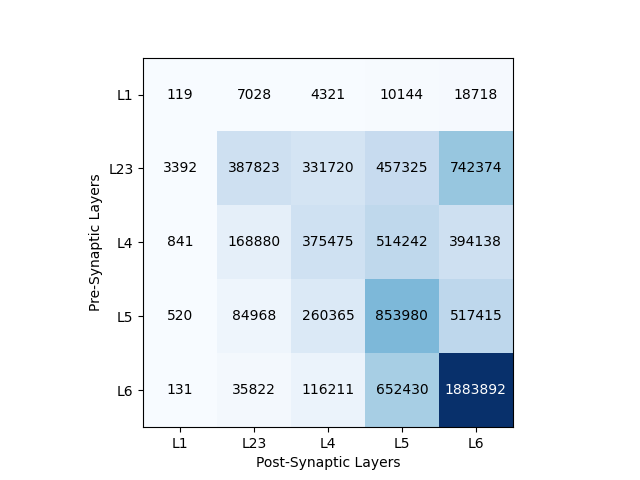
\includegraphics[width=7cm]{GC/heat_map_layer_GC.png} }}%
    \caption{Connectivity by block of the random graph $\mathcal{G}_{GC}$ given by the GC Model}%
    \label{fig:example}%
\end{figure}
\subsubsection{Distance Distribution}
We have a comparison of the distance distributions for a realisation of the Geometric Configuration model and the Bio-M MC in Figure 23. We see from this graph that the TV distance is much lower here than with the \ER model and the Configuration model, with a mean TV distance of 0.3169 after 100 realisations. This is to be expected given the construction of this model. More details of this statistic are found in Section 6, Results.


\begin{figure}[H]
\begin{center}
\captionsetup{justification=centering}
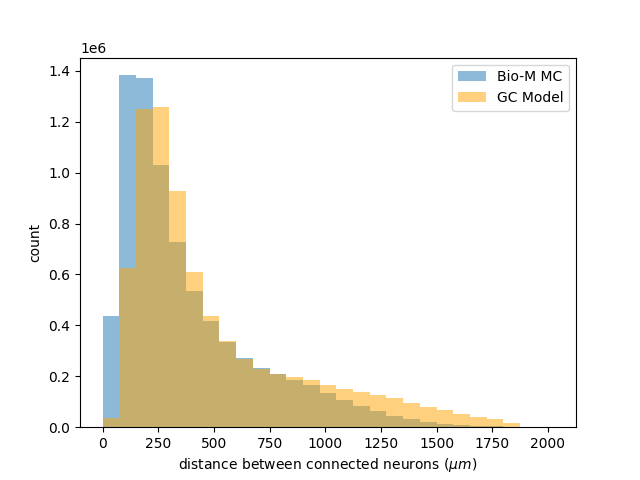
\includegraphics[width=12cm]{GC/GC_dist_distr.png}
\caption{Distance distribution of connected neurons for the random graph $\mathcal{G}_{GC}$}
\end{center}
\end{figure}

\subsubsection{Signed Degree of Neurons}
Figure 24 shows us that the in-degree and out-degree has been maintained, thereby showing that again the constraints of the  ``cut-permute-rewire'' \cite{WattsStrogatz1998} algorithm have been followed and that the graph representing the network is indeed finite.
\begin{figure}[H]%
    \centering
    \captionsetup{justification=centering}
    \subfloat[\centering Signed degree for each neuron ]{{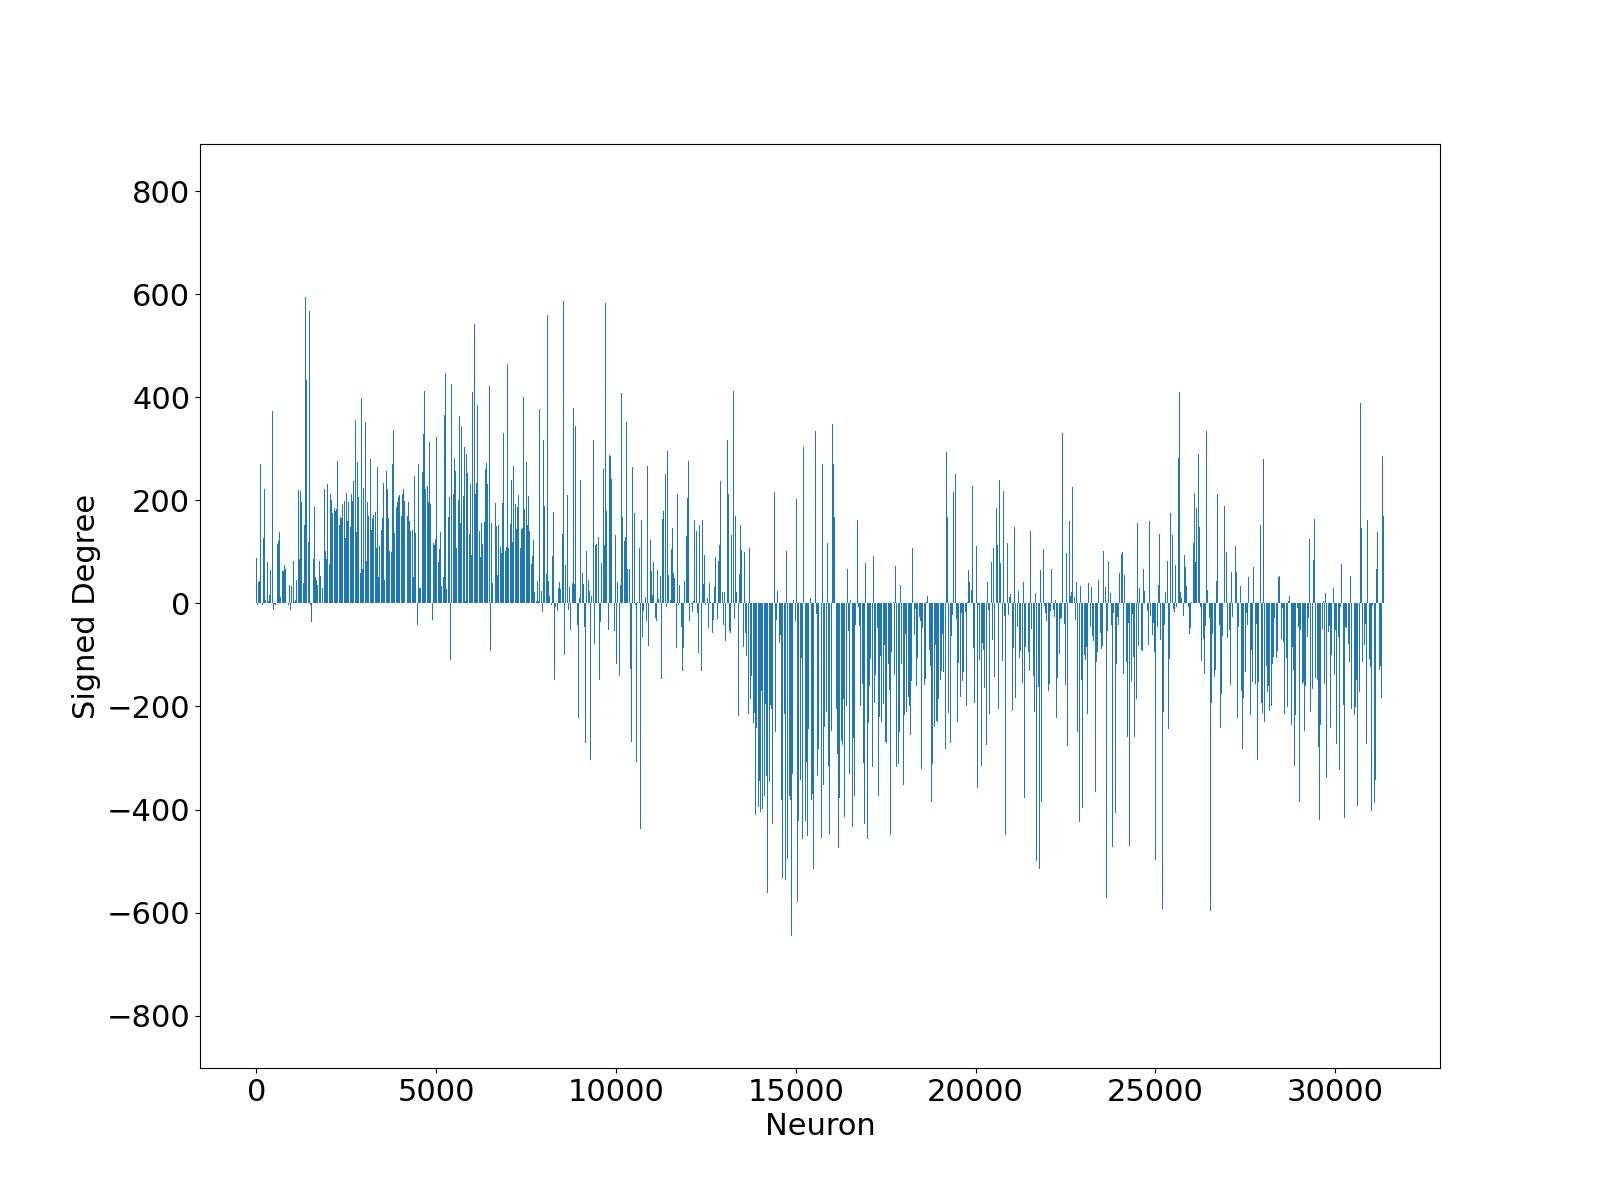
\includegraphics[width=7cm]{GC/GC_sd.png} }}%
    \qquad
    \subfloat[\centering Cumulative sum of the Signed Degree of the neurons in a realisation of the random graph $\mathcal{G}_{GC}$]{{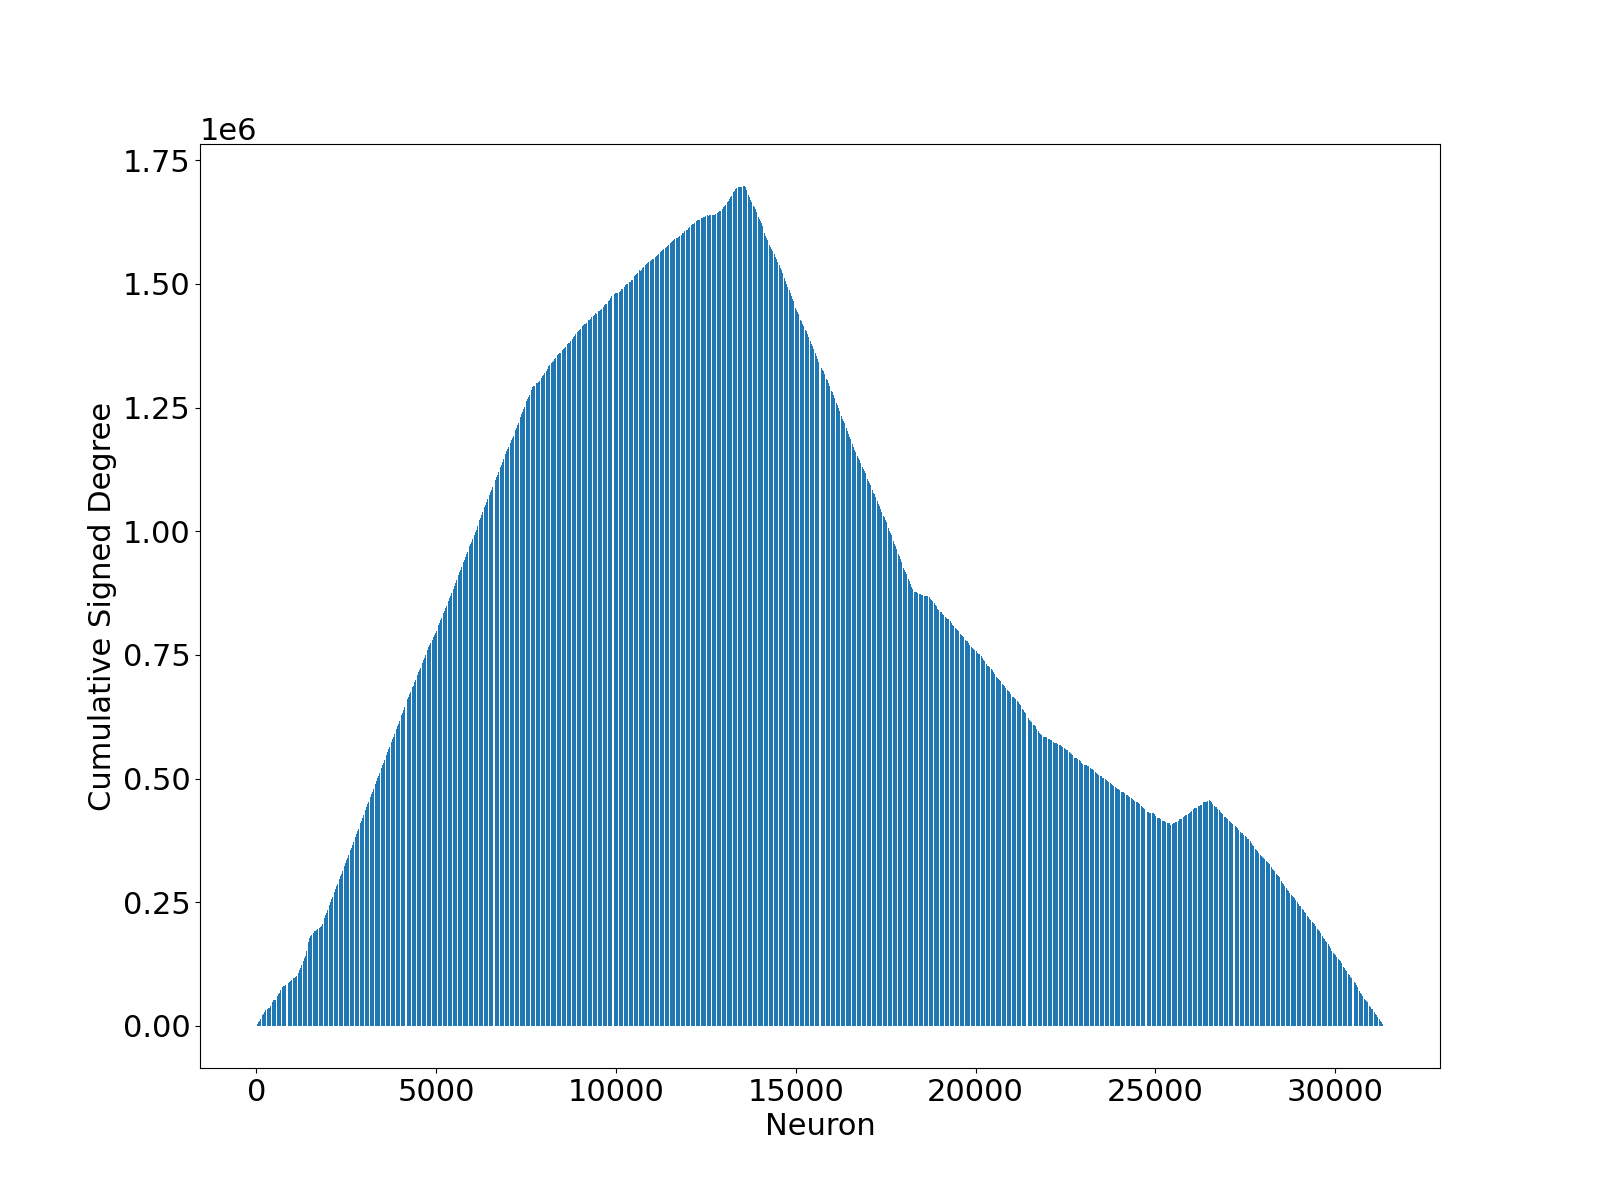
\includegraphics[width=7cm]{GC/cumsum_degree_GC.png} }}%
    \caption{Neuron statistics for the random graph $\mathcal{G}_{GC}$}%
    \label{fig:example}%
\end{figure}



\newpage
\subsection{Block Configuration Model}
In this section, we describe the Block Configuration model. This model uses the biological constraint of splitting up the MC into blocks comprising pre-synaptic neurons in a layer, say $i$, to post-synaptic neurons in a layer, say $j$ and using the ``cut-permute-rewire'' \cite{WattsStrogatz1998} algorithm in each block so that the layer-specific in-degrees and out-degrees for each neuron in each block is preserved, thereby seeing to it that this also remains the case for the entire random graph $\mathcal{G}_{BC}$.

\subsubsection{Construction}
The Block Configuration model is a hybrid of both the General Biological model (discussed later) and the Configuration model. This model divides up the connectome by layer rather than by morphological type, as was the case in the General Biological model and uses the ``cut-permute-rewire'' \cite{WattsStrogatz1998} algorithm.

The construction process of the Block Configuration model begins with dividing up the MC into its 25 blocks, as shown in Figure 6. This means that we take a subset of vertices V and edges E from the Bio-M MC for each block. For each subset, we apply Algorithm 2. The resulting ordered sets $u^\prime$ and $v$ are then stored until the algorithm has been applied to all 25 blocks. On completion, these 25 blocks containing the ordered sets of vertices, are then used to construct a realisation of the random graph $\mathcal{G_{BC}}$.


\begin{figure}[H]
\begin{center}
\captionsetup{justification=centering}
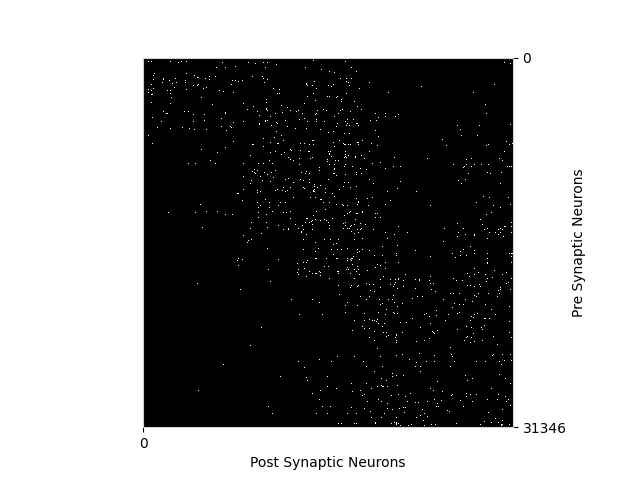
\includegraphics[width=12cm]{BC/matrix_Block_Configuration.png}
\caption{Adjacency Matrix $M$ representing a realisation of the random graph $\mathcal{G}_{BC}$}
\end{center}
\end{figure}

\subsubsection{Block Layouts}
Given that we have subdivided the MC into 25 blocks on a layer by layer basis, the number of edges contained in each block will be precisely the same as the Bio-M MC. This is shown in Section 6, where we detail the TV distance for Block-Wise Edge Densities between this model and the Bio-M MC. Likewise with the Configuration Model and the Geometric Configuration Model previously, we observe pairwise neurons with multiple connections in the same direction.
\begin{figure}[H]%
    \centering
    \captionsetup{justification=centering}
    \subfloat[\centering Block-Wise Edge Densities]{{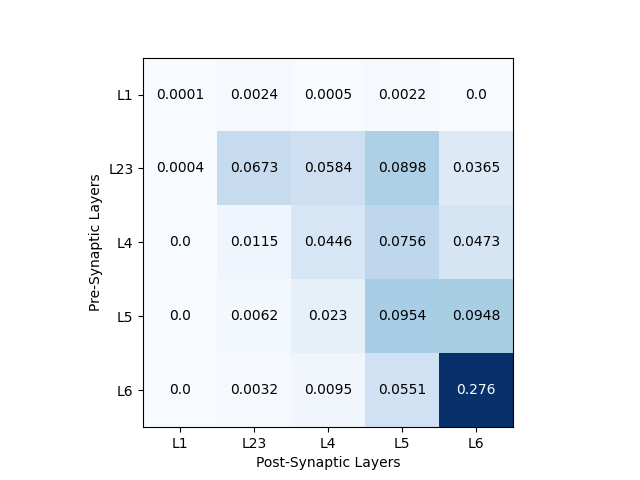
\includegraphics[width=7cm]{BC/heat_map_layer_bc_test.png} }}%
    \qquad
    \subfloat[\centering Block-Wise Edge Counts ]{{\includegraphics[width=7cm]{BC/heat_map_layer_Block.png} }}%
    \caption{Connectivity by block of the random graph $\mathcal{G}_{BC}$ given by the BC model}%
    \label{fig:example}%
\end{figure}
\subsubsection{Distance Distribution}
After 100 realisations of the Block Configuration model were observed, this yielded a mean TV distance of 0.3937. This is a large improvement on the \ER model and the Configuration model, however, weaker than the GC Model. Despite not allowing for a geometrical constraint here in terms of how a pair of neurons connect, it is clear that by dividing up the MC into these blocks plays a similar role in geometrically constraining the connections since we are only able to rearrange the connections in these specific blocks.
\begin{figure}[H]
\begin{center}
\captionsetup{justification=centering}
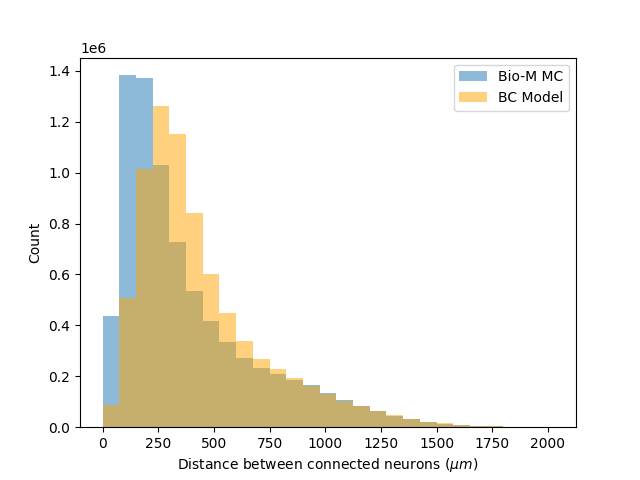
\includegraphics[width=12cm]{BC/Block_dist_distr.png}
\caption{Distance distribution of connected neurons for the random graph $\mathcal{G}_{BC}$}
\end{center}
\end{figure}

\subsubsection{Signed Degree of Neurons}
As mentioned at the head of this subsection, we have the same in-degrees and out-degrees for each neuron in each block and thereby ensuring the case for the whole random graph. \begin{figure}[H]%
    \centering
    \captionsetup{justification=centering}
    \subfloat[\centering  Signed Degree of each Neuron]{{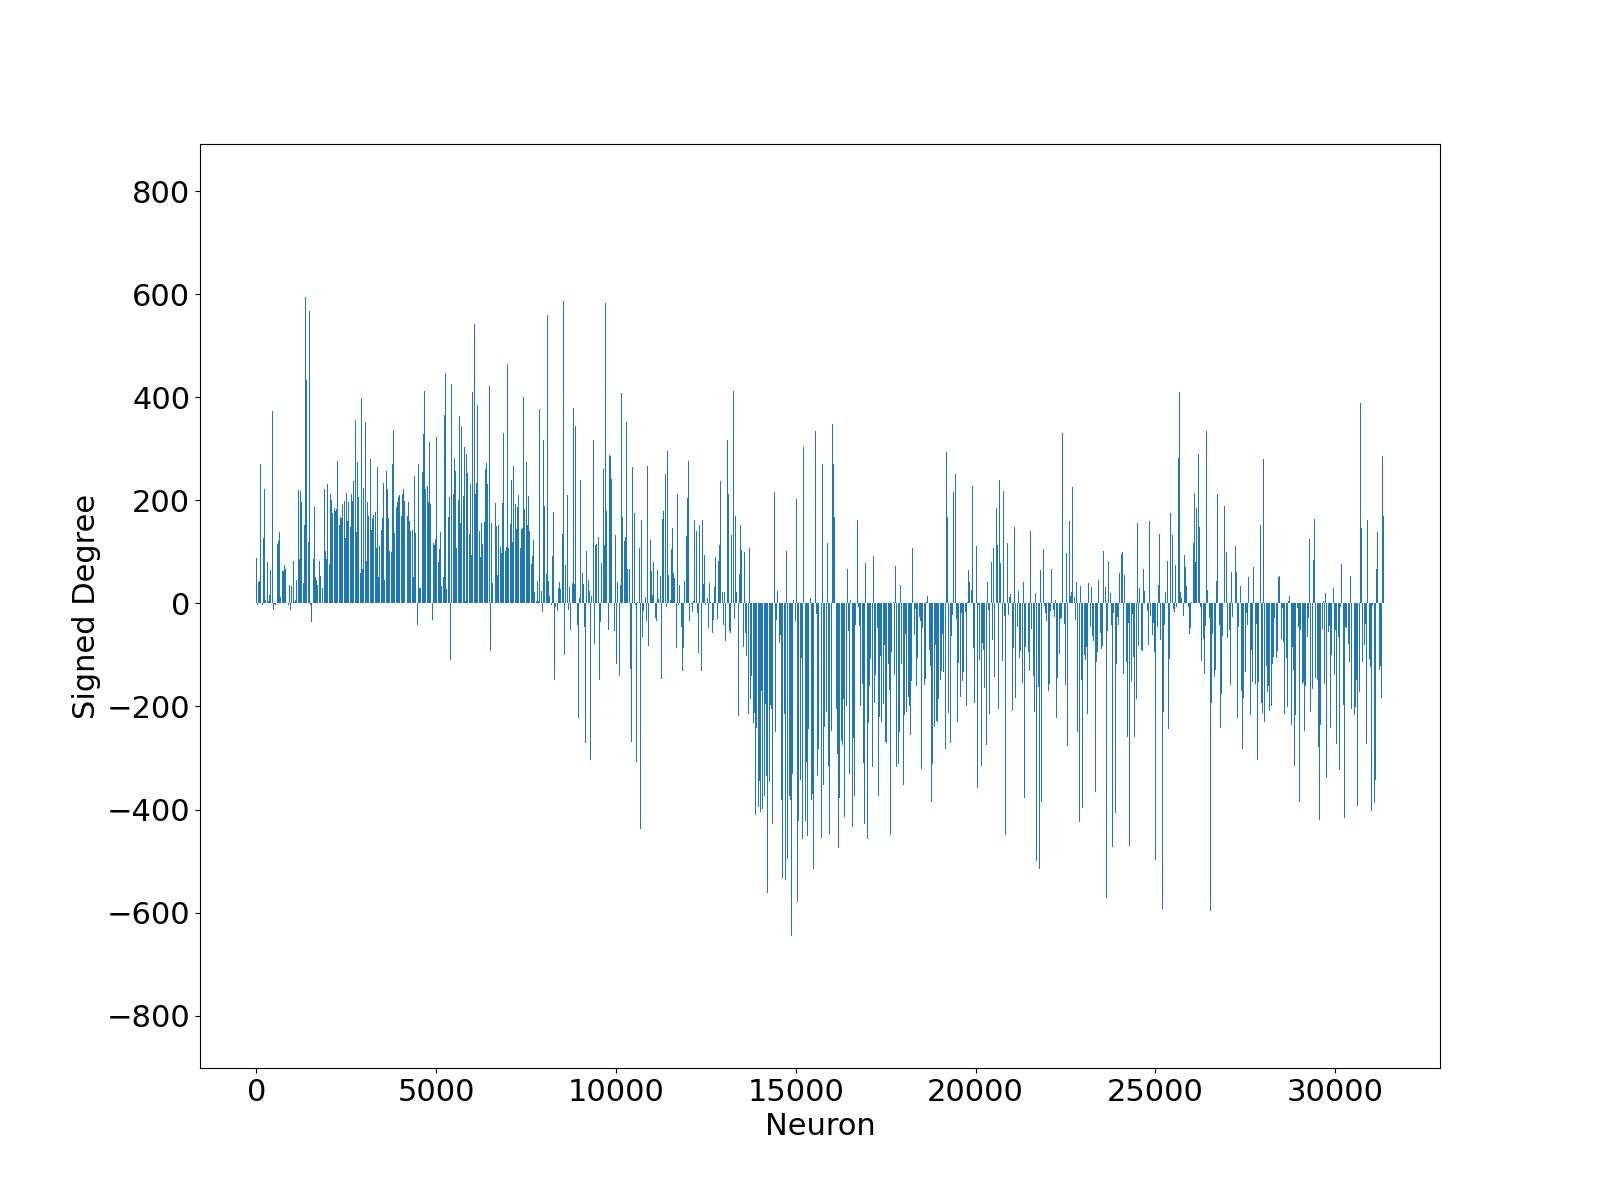
\includegraphics[width=7cm]{BC/Block_Configuration_sd.png} }}%
    \qquad
    \subfloat[\centering Cumulative sum of the Signed Degree of the neurons in a realisation of the random graph $\mathcal{G}_{BC}$ ]{{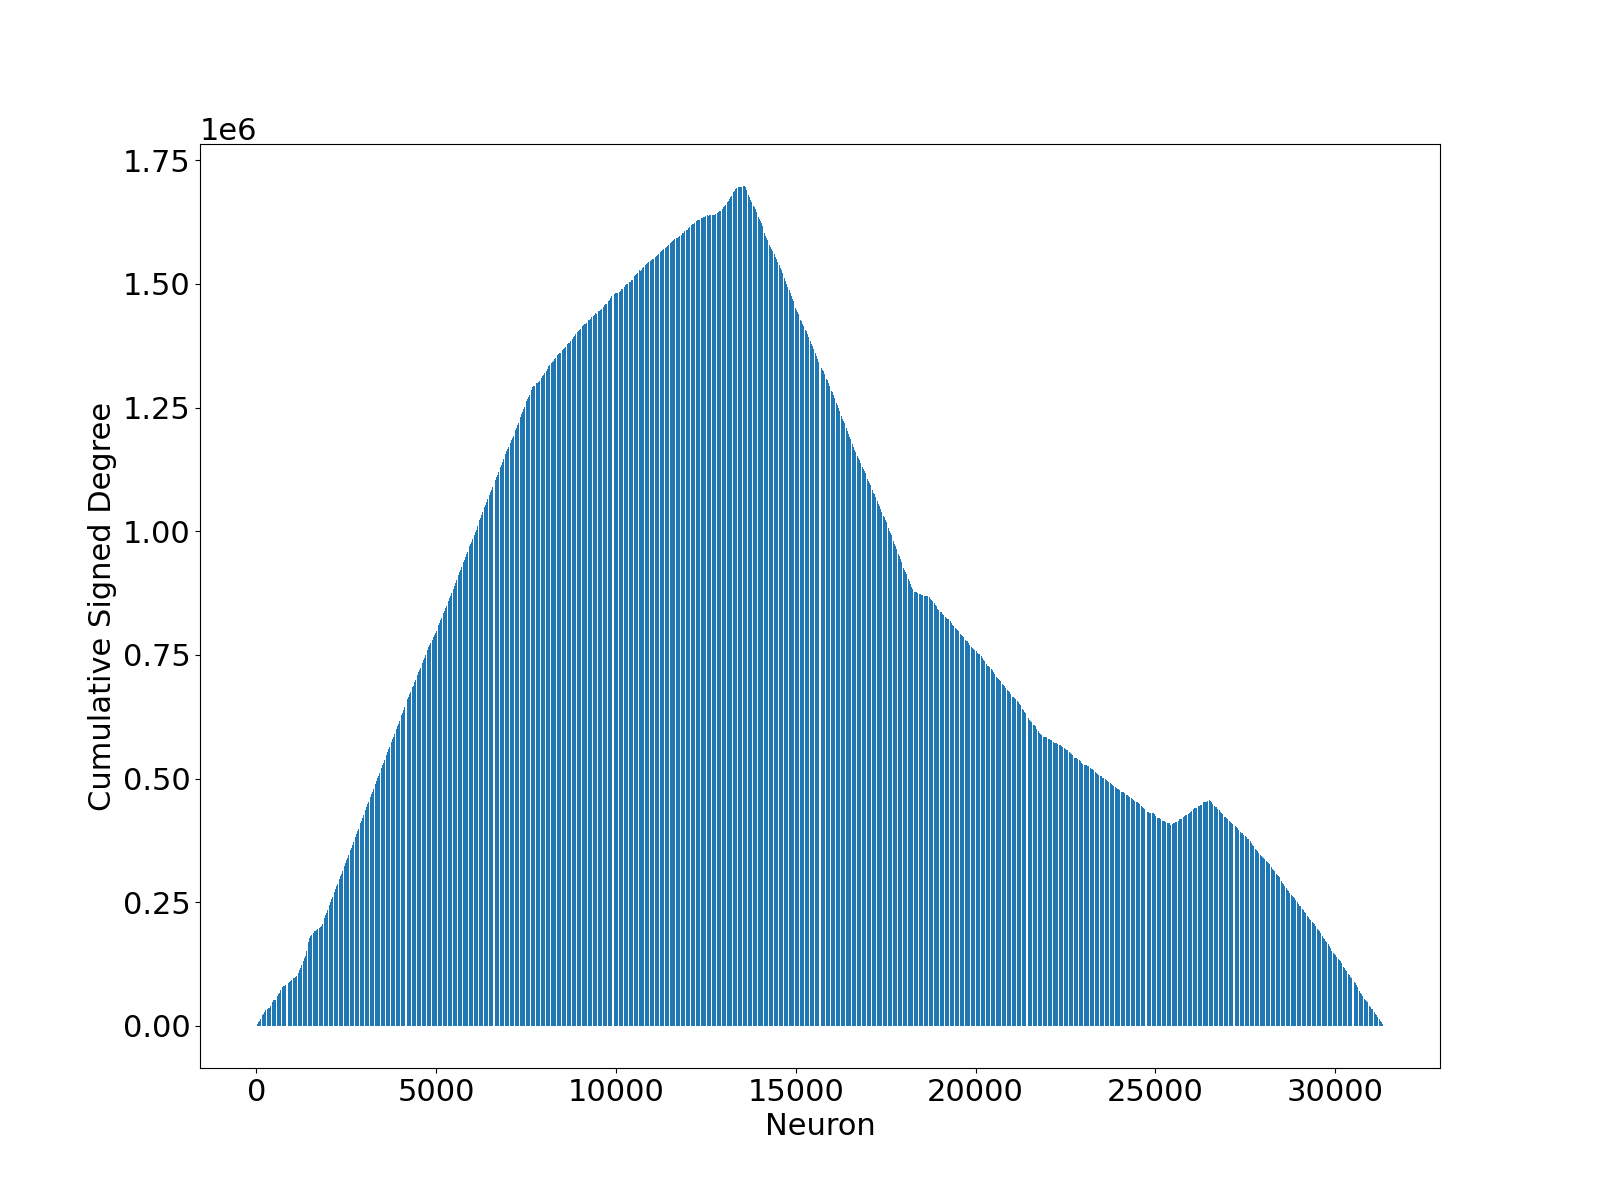
\includegraphics[width=7cm]{BC/cumsum_degree_Block_Configuration.png} }}%
    \caption{Neuron statistics for the random graph $\mathcal{G}_{BC}$}%
    \label{fig:example}%
\end{figure}

\newpage

\subsection{Block Geometric Configuration Model}
The Block Geometric Configuration model uses both the ``cut-permute-rewire'' \cite{WattsStrogatz1998} algorithm as well as the geometric constraint as mentioned in the GC model with a slight variation to it here.
\subsubsection{Construction}
The final model that we have is the Block Geometric Configuration model. The first part of the construction process, is to divide the MC into blocks, as was the case for the Block Configuration model. The second part of the process, is to then compute the pairwise distances of connected neurons in each block. That is, we take the subset of vertices and edges in each block, and compute the distances between these neurons. We then apply Algorithm 2 to each block and return the corresponding subsets $u^\prime$ and $v$. Upon completion of all 25 blocks, we can then use these ordered sets of vertices to construct a realisation of the random graph model $\mathcal{G_{BGC}}$. Thus, $\mathcal{G_{BGC}}$ not only preserves the in-degrees and out-degrees layer-specifically for each neuron but also the probability of connecting neurons based on the empirical pairwise distances of connected neurons.

\begin{figure}[H]
\begin{center}
\captionsetup{justification=centering}
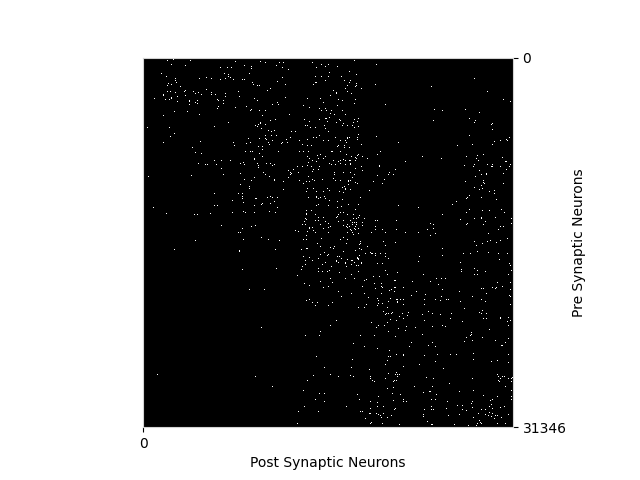
\includegraphics[width=12cm]{GBC/matrix_BGC.png}
\caption{Adjacency Matrix $M$ representing a realisation of the random graph $\mathcal{G}_{BGC}$}
\end{center}
\end{figure}


\subsubsection{Block Layouts}
Just as we saw for the Block Configuration model, each Block-Wise Edge density gives a TV distance of 0 to the Bio-M MC. As you will see from Figure 30, the values match that of the Bio-M MC. This, like the Block Configuration model has been achieved since all edge shuffling has occurred within these blocks that we are splitting the MC up into.

\begin{figure}[H]%
    \centering
    \captionsetup{justification=centering}
    \subfloat[\centering Proportion of connections in each block ]{{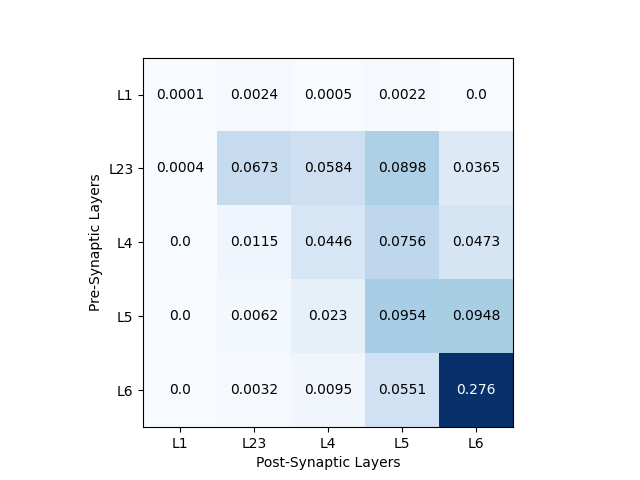
\includegraphics[width=7cm]{GBC/heat_map_layer_bgc_test.png} }}%
    \qquad
    \subfloat[\centering Total number of connections in each block ]{{\includegraphics[width=7cm]{GBC/heat_map_layer_Block.png} }}%
    \caption{Connectivity by block of the random graph $\mathcal{G}_{BGC}$ given by the BGC model}%
    \label{fig:example}%
\end{figure}

\subsubsection{Distance Distribution}

Figure 31 reveals a very similar distribution for the BGC model in comparison to the BC model. This, perhaps suggests that the geometric constraint has already been taken care of by splitting up the MC into these layer by layer blocks. Over 100 realisations of the BGC model yielded a mean TV distance of 0.3937. This is only marginally better than the BC model. Details of these differences are contained in Section 6, Results.

\begin{figure}[H]
\begin{center}
\captionsetup{justification=centering}
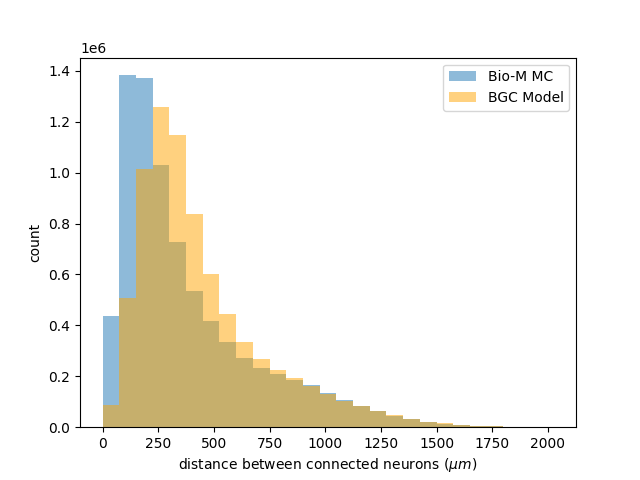
\includegraphics[width=12cm]{GBC/Block_dist_distr.png}
\caption{Distance distribution of connected neurons for the random graph $\mathcal{G}_{BGC}$}
\end{center}
\end{figure}

\subsubsection{Signed Degree of Neurons}
Just as with all the other models, we have the same in-degree and out-degree for each neuron as described by the plots in Figure 32.

\begin{figure}[H]%
    \centering
    \captionsetup{justification=centering}
    \subfloat[\centering Signed Degree of each Neuron]{{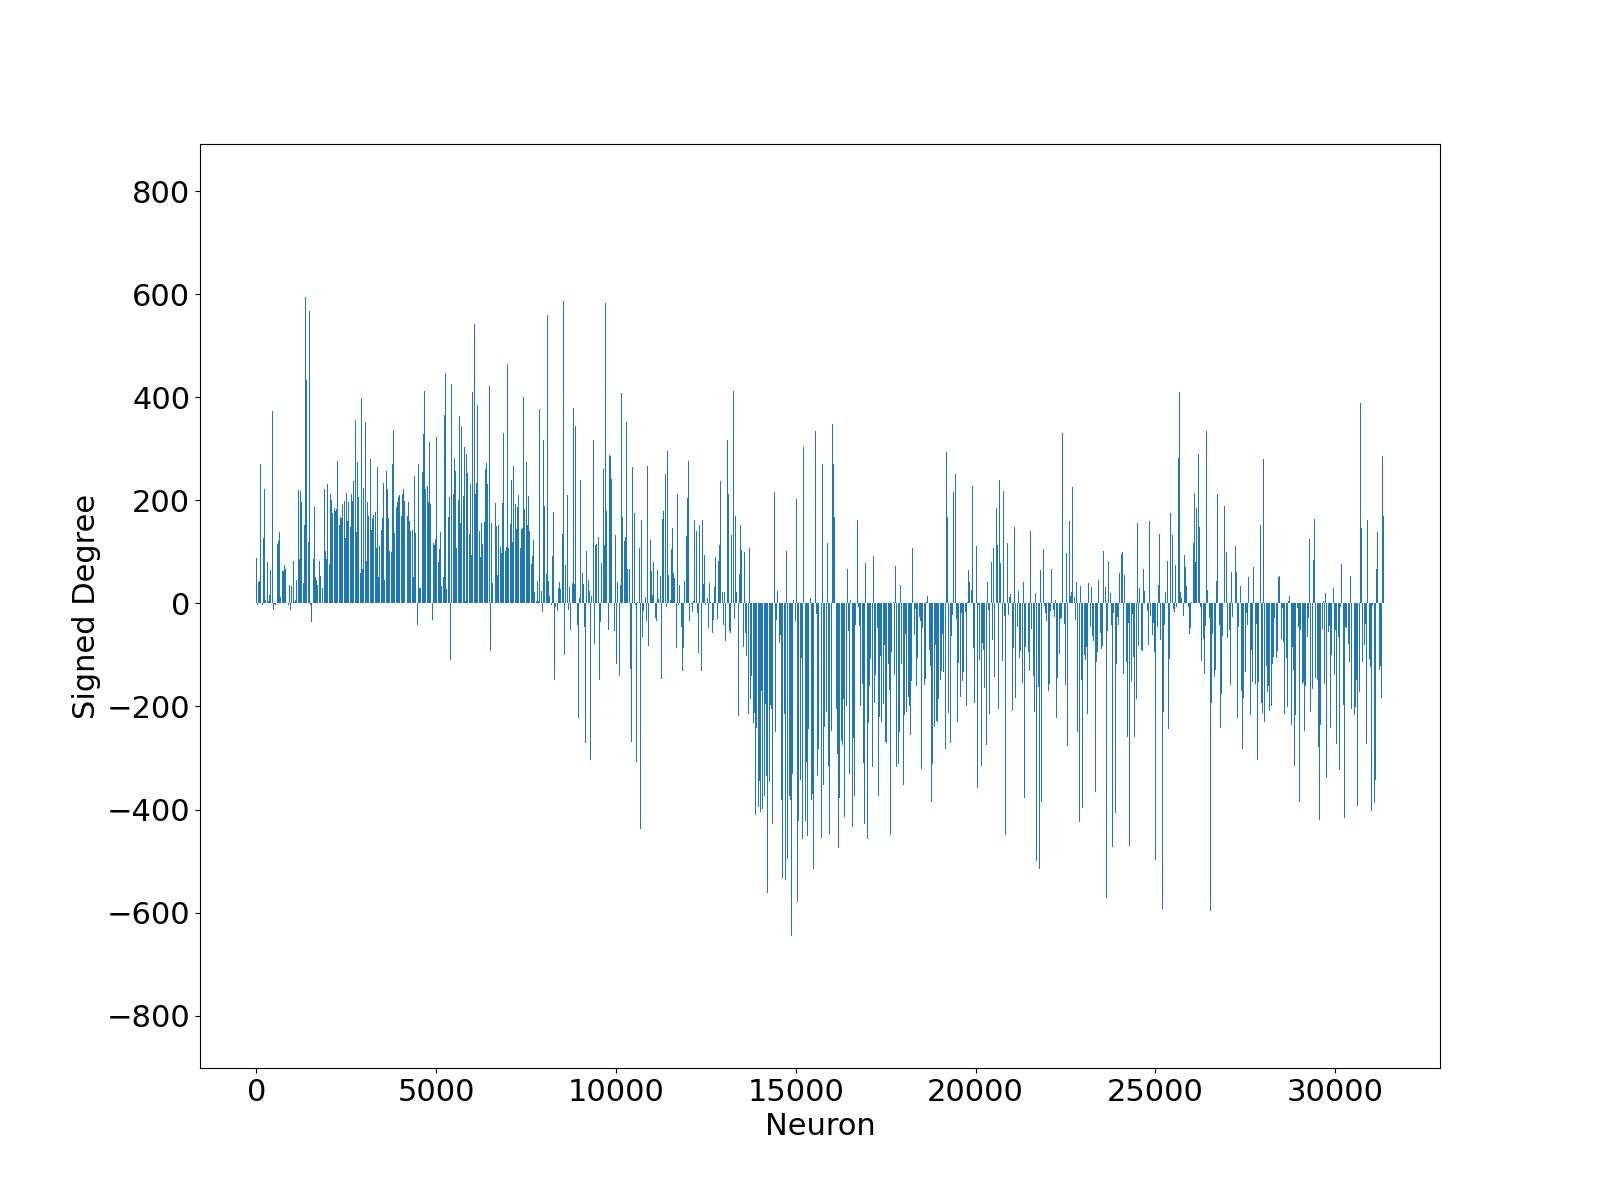
\includegraphics[width=7cm]{GBC/BGC_sd.png} }}%
    \qquad
    \subfloat[\centering Cumulative sum of the Signed Degree of the neurons in a realisation of the random graph $\mathcal{G}_{BGC}$]{{\includegraphics[width=7cm]{GBC/cumsum_degree_BGC.png} }}%
    \caption{Neuron statistics for the random graph $\mathcal{G}_{BGC}$}%
    \label{fig:example}%
\end{figure}



\newpage
\subsection{General Biological Model}
\subsubsection{The Model}
The General Biological model is the model that is proposed in the Frontiers article \cite{Reimann_2017}.

\begin{figure}[H]
\begin{center}
\captionsetup{justification=centering}
\includegraphics[width=12cm]{GB/matrix_general_biol.png}
\caption{Adjacency Matrix $M$ representing a realisation of the random graph $\mathcal{G}_{GB}$}
\end{center}
\end{figure}

This model subdivides the MC into 3025 sub-matrices which represent each morphological neuron type from pre-synaptic to post-synaptic neurons. That is, we have 55 different morphological neuron types. Now, within these sub-matrices, we compute the distances between all pairwise neurons. These distances get binned, as mentioned in Section 4.1.3, in to bin sizes of 75$\mu$m. Now, within these bins, we then shuffle the connections, so that a distance is preserved. We can see this diagrammatically in Figure 35. When the shuffling is completed, the sub-matrices are reassembled to form a complete matrix which now represents a realisation of the random graph $\mathcal{G}_{GB}$ given by the General Biological model.

\begin{figure}[H]%
    \centering
    \captionsetup{justification=centering}
    \subfloat[\centering Connections in each morphological block]{{\includegraphics[width=7cm]{GB/heat_map_morph_layer_general_biol.png} }}%
    \qquad
    \subfloat[\centering A closer look at the morphological block L1\_DAC ]{{\includegraphics[width=7cm]{GB/L1_DAC.png} }}%
    \caption{Connectivity of GB Model}%
    \label{fig:example}%
\end{figure}

\begin{figure}[H]%
    \centering
    \captionsetup{justification=centering}
    \subfloat[\centering Sample of connected graph before shuffling]{{\includegraphics[width=7cm]{GB/before.png} }}%
    \qquad
    \subfloat[\centering The same sample after shuffling ]{{\includegraphics[width=7cm]{GB/after.png} }}%
    \caption{An example of a block before shuffling connections and after}%
    \label{fig:example}%
\end{figure}
Figure 34(a) represents the number of connections in each block. The blocks are split into morphological type. As we can see by the bar on the right hand side, darker shades show a block that is highly populated with connections and a lighter block representing a less populated block of connections.
Figure 34(b) gives a representation of an individual morphological block, in this case L1 DAC, Layer 1 - Descending Axonal Collaterals, where we see pairwise neuron distances computed and binned according to a bin size of 75$\mu$m. The leading diagonal is the brightest shade of yellow and represents the smallest bin, that is a distance of 0$\mu$m and therefore are discounted, since they represent self-loops which do not exist. This leaves the remaining shades to be shuffled in each respective group.
Figure 35(a) and 35(b) represent a sample shuffling of connections, whereby the connections and non-connections are shuffled within their respective bins as defined by the shades.
\subsubsection{Block Layouts}
Now, by restricting the connection shuffling to morphological neuron type blocks, which are subsets of the layer by layer blocks, we are able to maintain a Block-Wise Edge density that is consistent with the Bio-M MC. Therefore, giving us a TV distance for Block-Wise Edge Densities of 0.

\begin{figure}[H]%
    \centering
    \captionsetup{justification=centering}
    \subfloat[\centering Block-Wise Edge Densities]{{\includegraphics[width=7cm]{GB/heat_map_layer_gb_test.png} }}%
    \qquad
    \subfloat[\centering  Block-Wise Edge Counts ]{{\includegraphics[width=7cm]{GB/heat_map_layer_general_biol.png} }}%
    \caption{Connectivity by block of the random graph $\mathcal{G}_{GB}$ given by the GB model}%
    \label{fig:example}%
\end{figure}

\subsubsection{Distance Distributions}
Figure 37 shows that with distance-dependence taken into account in the form of keeping bin sizes to a maximum size of $75\mu$m, we are able to maintain the exact same distribution as that of the Bio-M MC. In fact, we get a mean TV distance over 100 realisations, to be $\epsilon$. That is to say that the difference is statistically insignificant as a non-zero value occurred but once and was of the order $\epsilon < 1\times10^{-7}$. The details of the exact value is given in Section 6, Results.

\begin{figure}[H]
\begin{center}
\captionsetup{justification=centering}
\includegraphics[width=12cm]{GB/general_biol_dist_distr.png}
\caption{Distance distribution of connected neurons for the random graph $\mathcal{G}_{GB}$}
\end{center}
\end{figure}

\subsubsection{Signed Degree of Neurons}
One curiosity that occurred when constructing the random graph for the General Biological model was the directionality upon computing the cumulative sum. This exhibited a different path to that of all other models, and hence why it is shown in Figure 38(b). The underlying reason for this will be that whilst the construction process restricted the MC into blocks of morphological type and shuffled connections here, the shuffling wasn't based on the pre-existing connections in the MC, but rather the distances between all neurons within each block and therefore creating entirely new sets of pre-synaptic and post-synaptic neurons. This therefore, does not preserve the in-degree and out-degree of each neuron.
\begin{figure}[H]%
    \centering
    \captionsetup{justification=centering}
    \subfloat[\centering Cumulative Signed Degree]{{\includegraphics[width=7cm]{GB/cumsum_degree_general_biol.png} }}%
    \qquad
    \subfloat[\centering Directionality]{{\includegraphics[width=7cm]{GB/overall_degree_general_biol_sd_2.png} }}%
    \caption{a sample of the cumulative signed degree and the directionality of the GB model}%
    \label{fig:example}%
\end{figure}

\newpage
\section{Results}
\subsection{Simplices}
The first set of topological statistics we look at are the simplices. These statistics describe the local connectivity of a random graph. The higher the dimension of a simplex and the more simplices observed in each dimension, the more complex the structure becomes. The higher the dimension of the simplex, the more ordered this structure becomes.

Beginning with the Bio-M MC, we observe large numbers of simplices across the dimensions that went as high as dimension 6. In dimensions 2 and 3, we see simplices of almost as many as 80 and 70 million respectively. 

The first model of comparison is the \ER model. This model is able to match the simplicial counts of the Bio-M MC in the $0^{th}$ and $1^{st}$ dimensions, however, with a lack of order applied to the model, the complexity and ordered structure diminishes, the higher the simplicial dimension we attain.

The second model, the General Biological model, as produced here \cite{Reimann_2017}, again matches the Bio-M MC in the $0^{th}$ and $1^{st}$ dimension. The number of $2^{nd}$ dimensional simplices observed here is somewhat larger than what has been produced by the \ER model. There are approximately 35 million 2-dimensional simplices and just below 10 million 3-dimensional simplices. These two dimensions in particular are a focus point for which to be able to compare the four models proposed here. 

The Configuration model, like all subsequent models, produced precisely the same number of $0^{th}$ and $1^{st}$ dimensional simplices as that of the \ER model and the General Biological model, since these describe a single vertex and a directed edge joining two vertices as part of an ordered set respectively. The first difference occurs with the 2-dimensional simplices. Of the four proposed models, the Configuration model produced, consistently, the fewest 2-dimensional simplices. We observed approximately 33.5 million each time, 3 million fewer than the General Biological model. There is almost the same difference in the number of simplices between the Configuration model and the General Biological model for simplices in the $3^{rd}$ dimension compared to the $2^{nd}$ dimension.

Applying the geometric constraint in the Geometric Configuration model saw an improvement in matching the complexity of the Bio-M MC for 2-dimensional and higher simplices when compared to the Configuration model and the General Biological model. This refinement in the model, allowed for the biggest jump in accuracy between models, showing as many as 5 million more 2-dimensional simplices than the Configuration model, and almost 3 million more in the $3^{rd}$ dimension. 

The next model, the Block Configuration model saw the application of a biological constraint. This constraint is the layer to layer interactions of the neurons. By applying this layer to layer constraint, we were able to further improve the model's likeness to the Bio-M MC. This model observed as many as 41 million 2-dimensional simplices and 8.5 million 3-dimensional simplices. This is an improvement in both dimensions from the Geometric Configuration model. 

The Block Geometric Configuration model produced a similar number of 2- and 3-dimensional simplices as the Block Configuration model. So, there was no significant improvement to the numbers in these dimensions. However, this model did produce some more complex simplicial structures. We observed simplices in dimensions as high as the $6^{th}$, matching that of the Bio-M MC, just not as numerous.

\begin{figure}[H]
\begin{center}
\captionsetup{justification=centering}
\includegraphics[height=8cm,width=12cm]{graph/simplices_zoomed.png}
\caption{Simplicial Comparisons}
\end{center}
\end{figure}



\subsection{Betti Numbers and Euler Characteristic}
We want to compare the global connectivity of each model. We do this with Betti Numbers. In particular, we want to compare this connectivity in the highest dimension for which each model observes a non-zero Betti Number. This occurs in dimension 3. We have below, a set of results for 100 realisations of each model to give ourselves a statistical range to work with. 

In figures 40-42, we have individual box-plots for each model, followed by a box-plot with all the models side by side. The reason behind this can be observed with the scales used in each individual box-plot. We begin with the \ER model observing anywhere between 0 and 10 $3^{rd}$ dimensional Betti Numbers, all the way up to the Geometric model observing approximately $30,000$. Given that Betti Numbers is a count for the organisation of the structure of the graph, we can see that with a geometric constraint applied to the network, this enables the structure to maintain a lot more ordered structure than without this constraint. This appears more apparent between the Configuration model and the Geometric Configuration model than the respective Block models. This would suggest that the bigger the volume, the more important a geometric constraint is when simulating the connectivity of neurons.

\begin{figure}[H]%
    \centering
    \captionsetup{justification=centering}
    \subfloat[\centering \ER Model]{{\includegraphics[width=7cm]{graph/betti3_er.png} }}%
    \qquad
    \subfloat[\centering Configuration Model]{{\includegraphics[width=7cm]{graph/betti3_conf.png} }}%
    \caption{Box-plots of Betti Numbers observed in the $3^{rd}$ dimension for the models}%
    \label{fig:example}%
\end{figure}

\begin{figure}[H]%
    \centering
    \captionsetup{justification=centering}
    \subfloat[\centering Geometric Configuration Model]{{\includegraphics[width=7cm]{graph/betti3_geo.png} }}%
    \qquad
    \subfloat[\centering Block Configuration Model]{{\includegraphics[width=7cm]{graph/betti3_block_conf.png} }}%
    \caption{Box-plots of Betti Numbers observed in the $3^{rd}$ dimension for the models}%
    \label{fig:example}%
\end{figure}

\begin{figure}[H]%
    \centering
    \captionsetup{justification=centering}
    \subfloat[\centering Block Geometric Configuration Model]{{\includegraphics[width=7cm]{graph/betti3_block_geo.png} }}%
    \qquad
    \subfloat[\centering All Models]{{\includegraphics[width=7cm]{graph/all_betti.png} }}%
    \caption{Box-plots of Betti Numbers observed in the $3^{rd}$ dimension for the models}%
    \label{fig:example}%
\end{figure}


We also compare the $3^{rd}$ Betti Number with the Euler Characteristic for our 4 models. We can see that they cluster together within each model with a larger variation in the Betti Number. The block models observed similar values with respect to one another, especially in comparison to the other two models. The size of the graph can clearly give large differences in their clustered values as we see from the Configuration and Geometric Configuration models. 

\begin{figure}[H]
\begin{center}
\captionsetup{justification=centering}
\includegraphics[width=12cm]{graph/bVe.png}
\caption{Betti number in dimension 3 against Euler characteristic}
\end{center}
\end{figure}

\subsection{Total Variation distance: Distance Distribution}
One of the statistics we mention in Section 2, Mathematical Preliminaries, is the Total Variation (TV) distance. We use this statistic to give us a measure of how well one model may fit to that of the Bio-M MC in various statistical measures. However, here, we use it to check the fit of distance distributions and in the next subsection, how well the Block-wise Edge densities fit for each model.

So, we ran 100 realisations of each model with the intent to see how well the distributions of each model fit the distribution of the Bio-M MC. Below, after 100 realisations of each model, we have a table of the mean of each distribution. 

We can see that the models observed a wide range of TV distances in relation to one another, with the \ER model being the weakest and the GB model being the strongest. As mentioned in their respective sections, the BC model and the BGC model observe remarkably similar TV distances when comparing to the Bio-M MC. The spread of values for each respective model, was rather small, suggesting some consistency in the way the models reconnect the neurons in the MC.
\begin{center}
 \begin{tabular}{| c | c |} 
 \hline
 \textbf{Model} & \textbf{Mean Total Variation distance}  \\ [0.5ex] 
 \hline
 \ER &  0.7092   \\ 
 \hline
 Configuration & 0.6595    \\
 \hline
 Geometric Configuration & 0.3169   \\
 \hline
 Block Configuration & 0.3939   \\  
 \hline
 Block Geometric Configuration & 0.3937 \\  
 \hline
 General Biological & 1.5341e-08  \\
 \hline
\end{tabular}
\end{center}

\begin{figure}[H]%
    \centering
    \captionsetup{justification=centering}
    \subfloat[\centering \ER Model ]{{\includegraphics[width=7cm]{results_imgs/erModel.png} }}%
    \qquad
    \subfloat[\centering Configuration Model]{{\includegraphics[width=7cm]{results_imgs/cModel.png} }}%
    \caption{Box-plots of observed total distance variation from each model to the Bio-M MC}%
    \label{fig:example}%
\end{figure}

\begin{figure}[H]%
    \centering
    \captionsetup{justification=centering}
    \subfloat[\centering Geometric Configuration Model]{{\includegraphics[width=7cm]{results_imgs/gcModel.png} }}%
    \qquad
    \subfloat[\centering Block Configuration Model]{{\includegraphics[width=7cm]{results_imgs/bcModel.png} }}%
    \caption{Box-plots of observed total distance variation from each model to the Bio-M MC}%
    \label{fig:example}%
\end{figure}

\begin{figure}[H]%
    \centering
    \captionsetup{justification=centering}
    \subfloat[\centering Block Geometric Configuration Model]{{\includegraphics[width=7cm]{results_imgs/bgcModel.png} }}%
    \qquad
    \subfloat[\centering General Biological Model]{{\includegraphics[width=7cm]{results_imgs/gbModel.png} }}%
    \caption{Box-plots of observed total distance variation from each model to the Bio-M MC}%
    \label{fig:example}%
\end{figure}
A note on the General Biological model from what we see in Figure 46(b) is that over the 100 realisations we obtained a TV distance greater than zero for one realisation. Given that this occurred only once and that the difference is insignificant, we do not concern ourselves with this. 

\subsection{Total Variation distance: Block-wise Edge Densities}
Here, we compare the Block-wise Edge densities between each model and the Bio-M MC. As we mentioned previously, there were 100 realisations of each model and each were compared to the Bio-M MC. To begin comparison, we compare each block and then sum over all blocks to ascertain the TV distance of each model to the Bio-M MC and where relevant, we then give a breakdown of TV distances, block by block.  

\begin{figure}[H]%
    \centering
    \captionsetup{justification=centering}
    \subfloat[\centering \ER Model]{{\includegraphics[width=7cm]{results_imgs/er_block_var.png} }}%
    \qquad
    \subfloat[\centering Configuration Model]{{\includegraphics[width=7cm]{results_imgs/conf1_overall.png} }}%
    \caption{Box-plots of observed total distance variation from each model to the Bio-M MC}%
    \label{fig:example}%
\end{figure}
Figure 47 shows us the \ER model and the Configuration model. Both models show a similar range of values, however, the range of values given by the Configuration model is closer to that of the Bio-M MC. This 0.12 improvement between models is somewhat significant, highlighting the importance to maintain the in-degrees and out-degrees of the respective neurons in an already observed MC. 

\begin{figure}[H]%
    \centering
    \captionsetup{justification=centering}
    \subfloat[\centering Geometric Configuration Model]{{\includegraphics[width=7cm]{results_imgs/gc1_overall.png} }}%
    \qquad
    \subfloat[\centering Block Configuration Model]{{\includegraphics[width=7cm]{results_imgs/bc_block_var.png} }}%
    \caption{Box-plots of observed total distance variation from each model to the Bio-M MC}%
    \label{fig:example}%
\end{figure}

Figure 48(a) highlights further the importance of a geometric constraint applied to the MC. The improvement of Block-wise Edge densities almost doubles from the Configuration model. Furthermore, we have no outliers in our range of values, showing that the model can statistically be more consistent with the Bio-M MC. The Block Configuration model exhibits no differences to the Bio-M MC as is the case for the BGC model and the GB model. This is since they rearrange connections within the layer by layer blocks or subsets of these (morphological blocks). 
\begin{figure}[H]%
    \centering
    \captionsetup{justification=centering}
    \subfloat[\centering Block Geometric Configuration Model]{{\includegraphics[width=7cm]{results_imgs/bgc_block_var.png} }}%
    \qquad
    \subfloat[\centering General Biological Model]{{\includegraphics[width=7cm]{results_imgs/GB_block_var.png} }}%
    \caption{Box-plots of observed total distance variation from each model to the Bio-M MC}%
    \label{fig:example}%
\end{figure}


\begin{figure}[H]
\begin{center}
\captionsetup{justification=centering}
\includegraphics[width=12cm]{results_imgs/er_bed.png}
\caption{Block-wise Edge Density Total Variation Distance Block by Block: \ER Model}
\end{center}
\end{figure}
The \ER model gives a range of TV distances for each block. The biggest occurring in L6 to L6. The smallest sets of values occur in the blocks that relate to Layer 1, whether it be the pre-synaptic set of neurons or the post-synaptic set of neurons.
\begin{figure}[H]
\begin{center}
\captionsetup{justification=centering}
\includegraphics[width=12cm]{results_imgs/conf_bed.png}
\caption{Block-wise Edge Density Total Variation Distance Block by Block: Configuration Model}
\end{center}
\end{figure}
Now, likewise with the \ER model, the Configuration Model observes the largest set of TV distances from L6-L6 and similarly much smaller values for L1, whether it be from pre-synaptic neurons or to post-synaptic neurons, the TV distance values here are just a lot smaller. 

\begin{figure}[H]
\begin{center}
\captionsetup{justification=centering}
\includegraphics[width=12cm]{results_imgs/gc_bed.png}
\caption{Block-wise Edge Density Total Variation Distance Block by Block: Geometric Configuration Model}
\end{center}
\end{figure}
As mentioned for the \ER model and the Configuration model, the smallest differences occur in relation to neurons in Layer 1 for the GC model. However, we note here that in fact, there is a large improvement to the difference in respect of the L6-L6 connections, where we only see a mean TV distance of approximately 0.025, a large improvement on the previous two models, highlighting the strength of the geometric constraint.


\subsection{Timings}
\begin{figure}[H]
\begin{center}
\captionsetup{justification=centering}
\includegraphics[width=12cm]{graph/timings.png}
\caption{Computation times for the random graphs}
\end{center}
\end{figure}

\begin{center}
 \begin{tabular}{| c | c | c | c |} 
 \hline
 \textbf{Model} & \textbf{Min(s)} & \textbf{Mean(s)} & \textbf{Max(s)} \\ [0.5ex] 
 \hline
 \ER & 5 & 5    & 5    \\ 
 \hline
 Configuration &  49.78 & 50.63  & 51.75   \\
 \hline
 Geometric Configuration & 854.87
 & 870.93 &  901.63   \\
 \hline
 Block Configuration & 34.77 & 34.01 & 35.55   \\ 
 \hline
 Block Geometric Configuration & 94.77
  & 97.55 & 99.89 \\  
 \hline
 General Biological & 420  & 426     & 432   \\
 \hline
\end{tabular}
\end{center}
Finally, we have our timings for the models. All of these were computed on the same machine, of which the details are listed below. However, there were slight differences in the methods between my models and that of the General Biological model and Bio-M MC. The General Biological model and Bio-M MC were computed first by converting the file formats from H5 to CSV and then converted to an NPY array, whereas my models just simply needed to take the saved NPY array.

A note on the geometrically constrained models is that they had a similar computation time up until approximately 80$\%$ completion and then slowed down significantly in order to connect the remaining vertices. Therefore the remaining 20$\%$ of connections took the majority of time to compute.
\newpage
\begin{lstlisting}[language=bash]
Architecture:                    x86_64
CPU op-mode(s):                  32-bit, 64-bit
Byte Order:                      Little Endian
Address sizes:                   43 bits physical, 48 bits virtual
CPU(s):                          12
On-line CPU(s) list:             0-11
Thread(s) per core:              2
Core(s) per socket:              6
Socket(s):                       1
NUMA node(s):                    1
Vendor ID:                       AuthenticAMD
CPU family:                      23
Model:                           113
Model name:                      AMD Ryzen 5 3600 6-Core Processor
Stepping:                        0
Frequency boost:                 enabled
CPU MHz:                         2199.811
CPU max MHz:                     3600,0000
CPU min MHz:                     2200,0000
BogoMIPS:                        7199.87
Virtualization:                  AMD-V
L1d cache:                       192 KiB
L1i cache:                       192 KiB
L2 cache:                        3 MiB
L3 cache:                        32 MiB
NUMA node0 CPU(s):               0-11
\end{lstlisting}






\newpage
\section{Conclusion}
\subsection{Summary}
The goal of this paper was to find a model that would represent the neural network as defined by the Bio-M MC as closely as possible through the use of topological statistics. Given the array of constraints that we could apply to the model, we chose to incrementally add these constraints to the models to see if there is improvement in each one. We found that each implementation had their own unique improvement. 

\subsection{Future Implementations}
A future implementation that could see an improvement in connectivity, especially on the local level, would be to consider a cloud connected model. The idea being that we take axon and dendrite lengths into account in the way where we add a volume around each neuron that has a certain axon and dendrite cloud covering, apply a probability of connection, then randomly select a connection until we have a matching amount of connections in the MC as the Bio-M MC and compare topological statistics as we have done above.

Further to this, there are multiple instantiations that we did not consider and if we had included them, this may give rise to models that could be better suited to these instantiations as compared to how they affected this instantiation (Bio-M).

\section{Acknowledgements}

This research was partially supported by the Wallenberg AI, Autonomous Systems and Software Program funded by Knut and Alice Wallenberg Foundation. 
The distributed computing infrastructure for this pjoject was supported by Databricks University Alliance with AWS credits.

Many thanks to Kathryn Hess, Svante Janson, Wojciech Chachólski, Martina Scolamiero, and Michael Reimann.





\newpage
\section{Appendix}
% \subsection{Python Scripts}
% \url{https://github.com/lamastex/working-manuscript-TopologicalDataAnalysisOnABrainNetwork}

\bibliographystyle{plain}
\bibliography{references}


\end{document}
